\chapter{Resultados}
%\noindent
O capítulo apresenta os resultados obtidos ao realizar os procedimentos especificados na metodologia. Etapas e especificações complementares são descritos com o intuito de facilitar o entendimento dos procedimentos executados.

\section{RTPPP com estação da RBMC}

Primeiramente, foi realizado um RTPPP utilizando a estação POAL da RMBC sem a especificação da antena utilizada pelo receptor. A ausência das informação da antena se deu pelo fato da versão mais atual do software utilizado (BNC 2.12) ter alterado o modo de inserção de tal informação em relação a versões anteriores (BNC 2.9). Na versão 2.12 as informações de antena devem ser inseridas juntamente com o arquivo de coordenadas.

Seguem os resultados:

\begin{figure}[H]
\centering
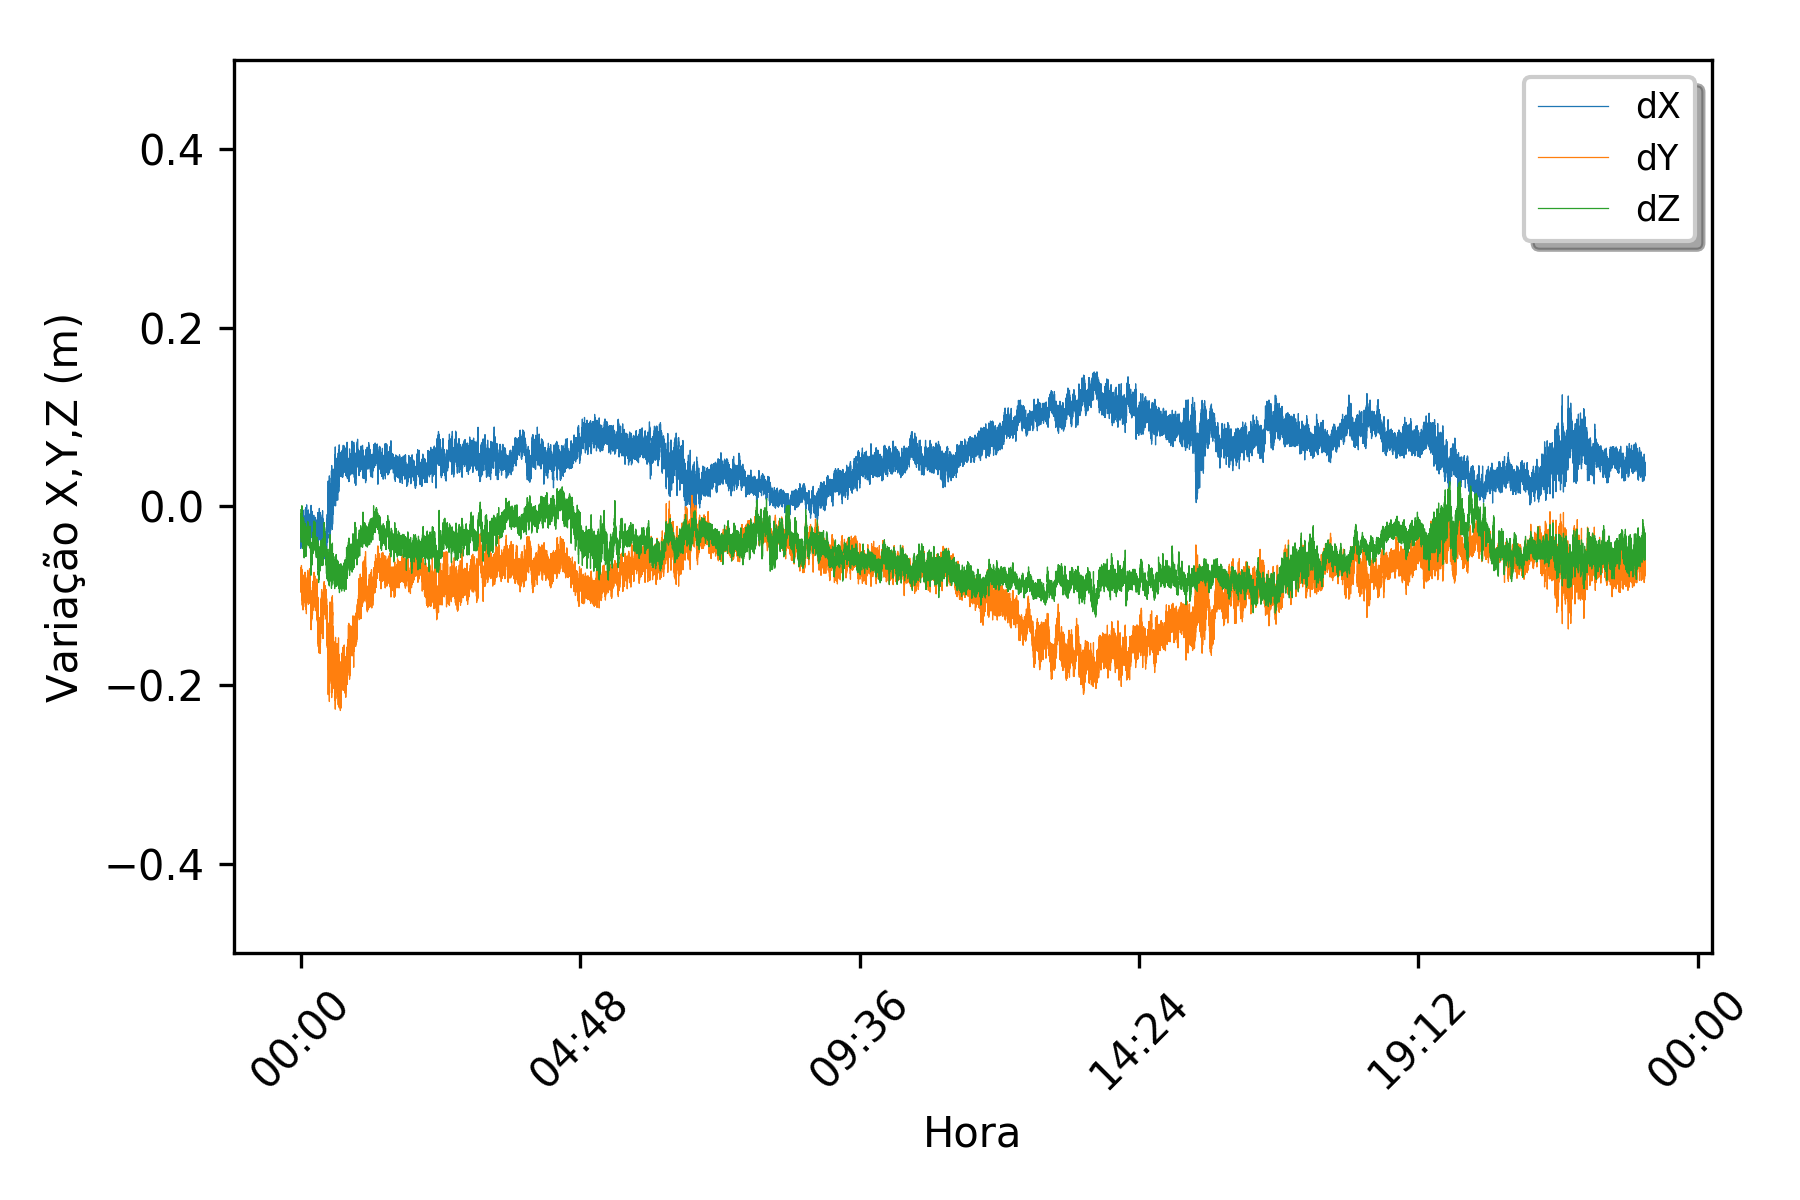
\includegraphics[scale=0.9]{data/Graphics/POAL20636/POAL20636_graphic_xyz.png}
\caption{Série temporal RTPPP - dX, dY, dZ.}
\label{rtppp1}
\end{figure}

As coordenadas utilizadas como referência para os cálculos de dX, dY e dZ para cada época foram as coordenadas obtidas em \cite{sirgascon} para a semana GPS 2065.

Pode-se observar na fig. \ref{rtppp1} que desde o início da coleta de dados o RTPPP apresentou variações relativamente pequenas nas componentes dX, dY, dZ; entretanto é possível observar uma tendência nas três componentes.

\begin{figure}[H]
\centering
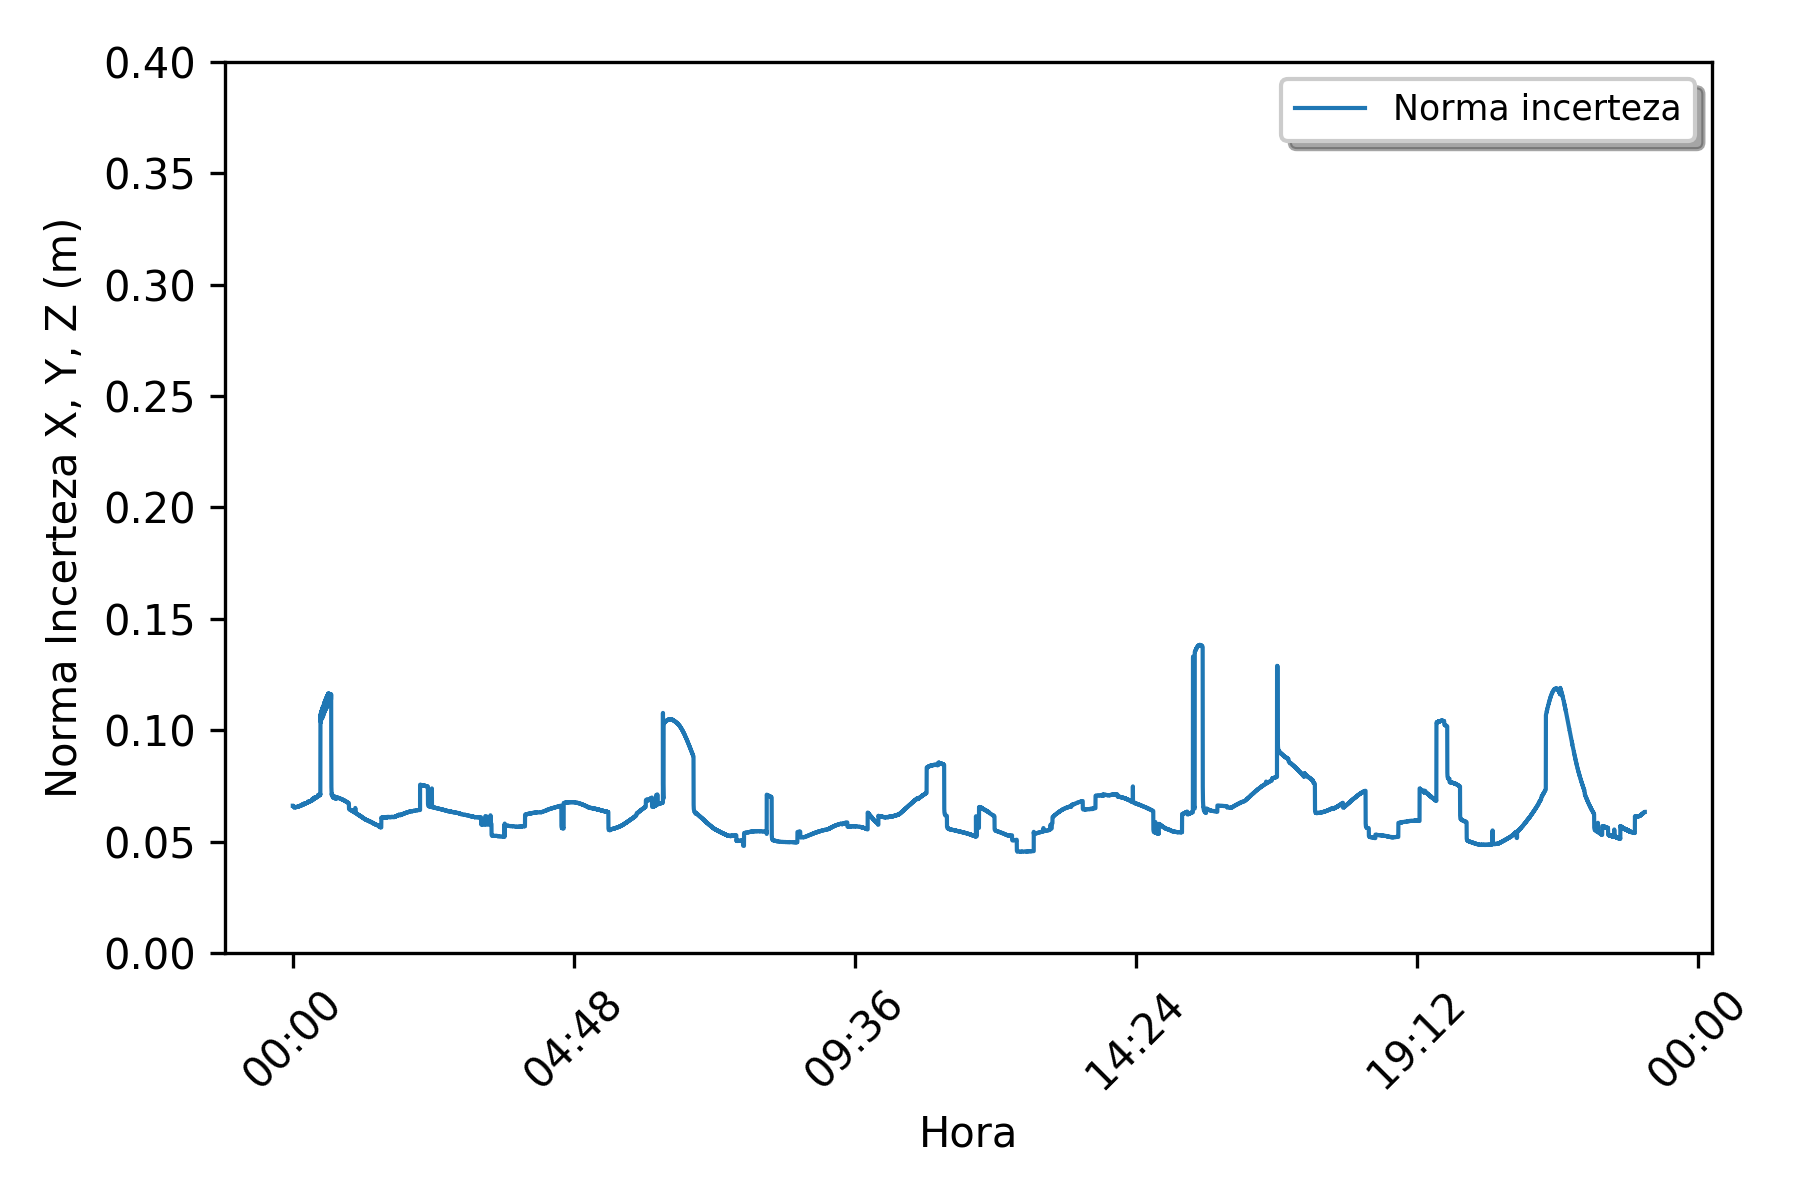
\includegraphics[scale=0.9]{data/Graphics/POAL20636/POAL20636_graphic_uncertainty.png}
\caption{Série temporal RTPPP - Incerteza das coordenadas X, Y, Z.}
\label{incert1}
\end{figure}

Pelo fato de estar-se realizando um PPP em tempo real, uma possibilidade para verificar a qualidade dos dados em tempo real é verificar a incerteza das coordenadas X, Y e Z que são obtidas em tempo real. A norma das incertezas das coordenadas X, Y e Z na fig. \ref{incert1} variou entre aproximadamente 5 e 14 cm.

\begin{figure}[H]
\centering
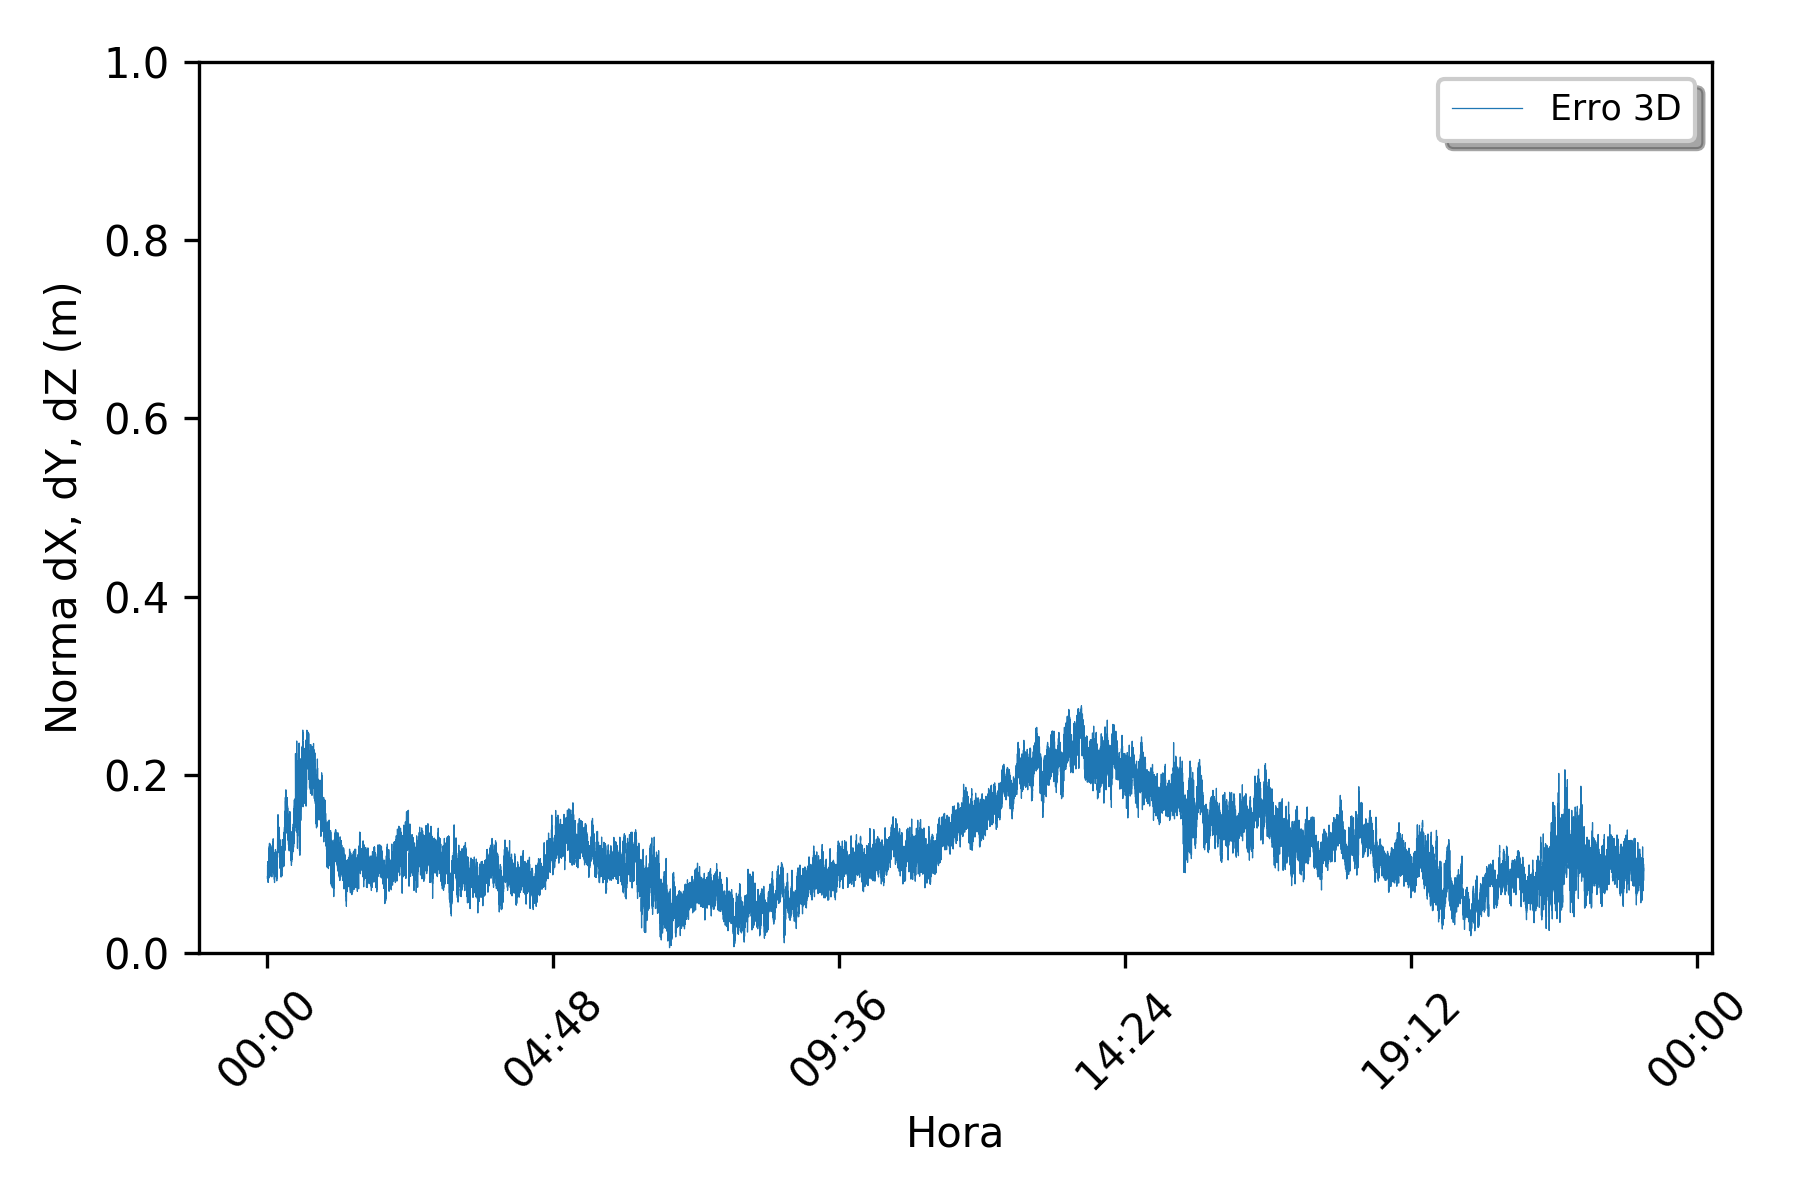
\includegraphics[scale=0.9]{data/Graphics/POAL20636/POAL20636_graphic_result.png}
\caption{Série temporal RTPPP - Resultante dX, dY, dZ.}
\label{result1}
\end{figure}

O erro médio quadrático do erro 3D deste levantamento foi de $0,126634$. Na fig. \ref{result1} pode-se observar que a norma do vetor resultante de dX, dY e dZ variou entre aproximadamente 22 cm e 37 cm. Tal variação é acima do esperado para um PPP mas provavelmente reflete as tendências causadas pela ausência de informações da antena do receptor.

Após isso, utilizando a mesma estação, realizou-se um RTPPP com a especificação da antena utilizada pelo receptor. A seguir os resultados:

\begin{figure}[H]
\centering
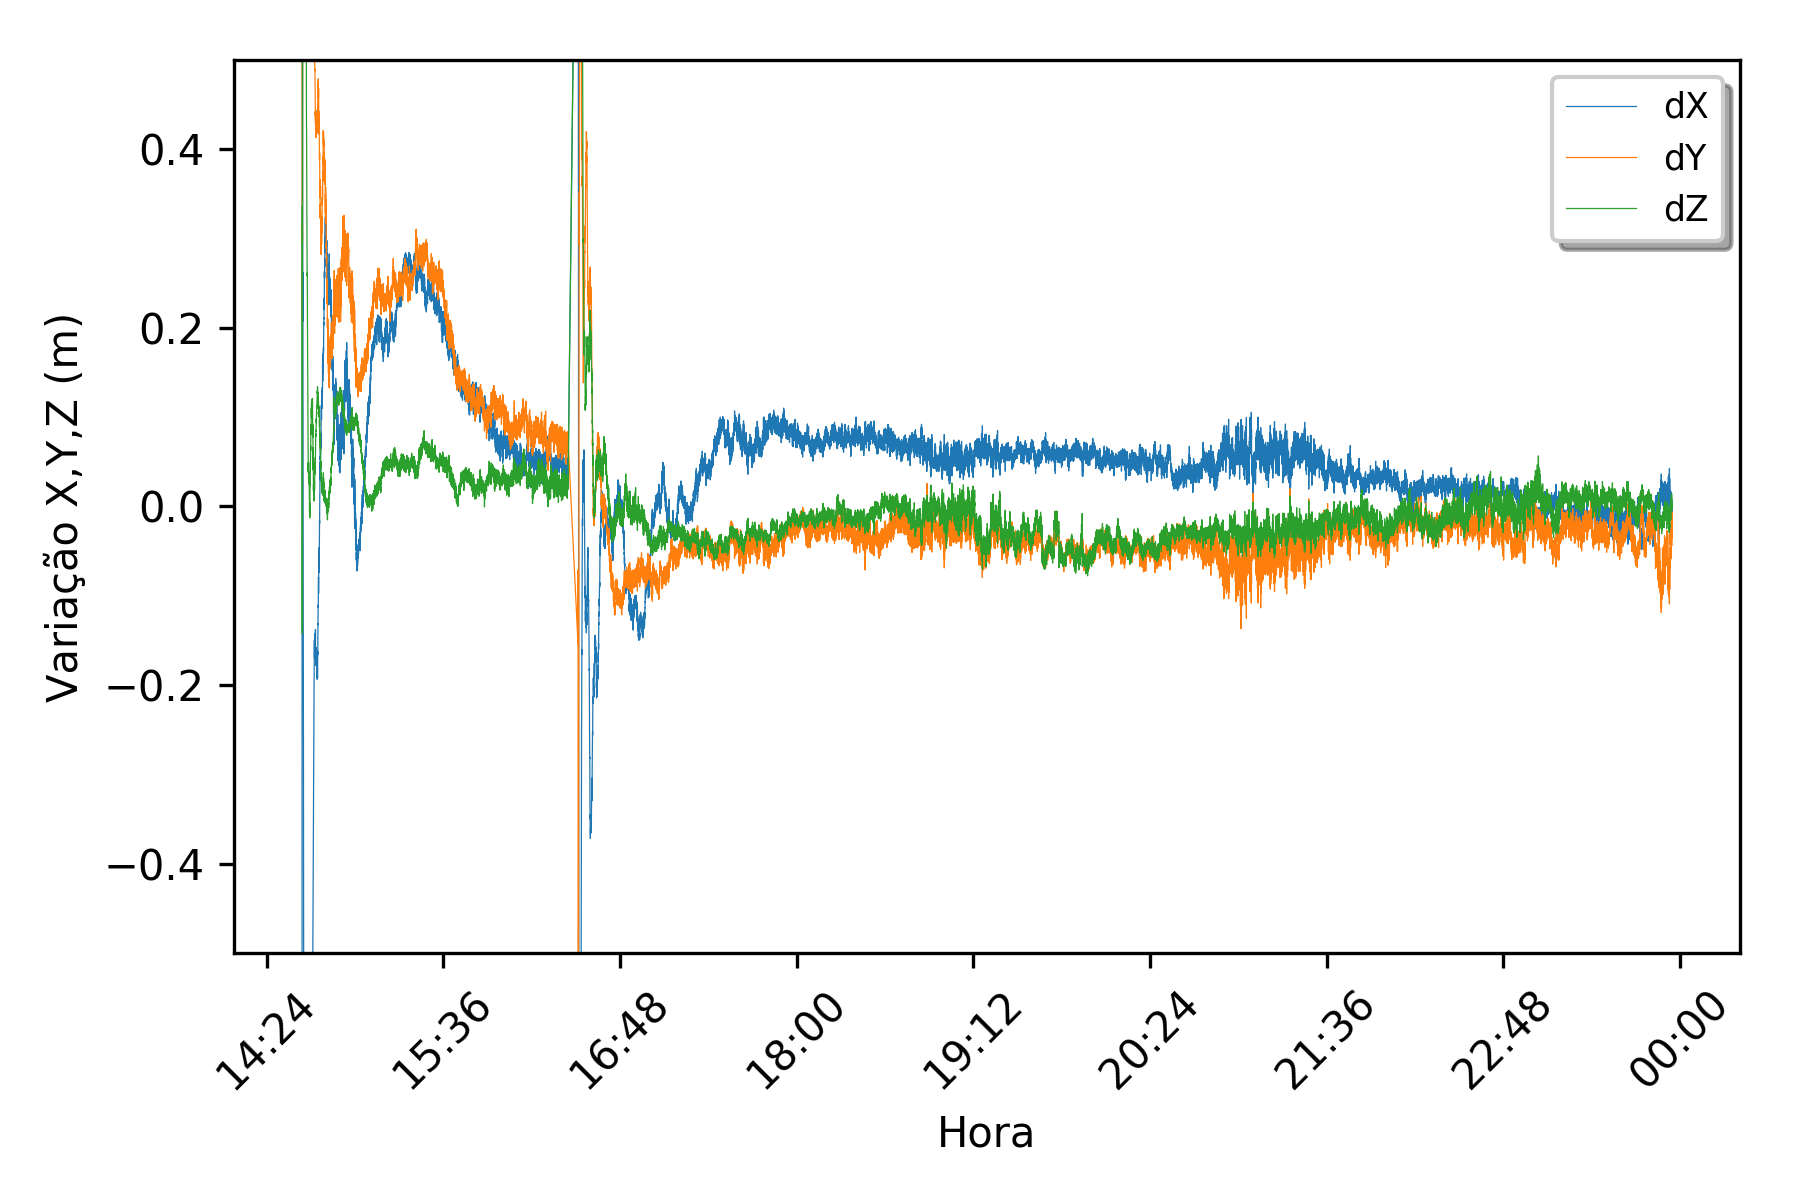
\includegraphics[scale=0.9]{data/Graphics/POAL20650/POAL20650_graphic_xyz.png}
\caption{Série temporal RTPPP - dX, dY, dZ.}
\label{rtppp2}
\end{figure}

Na fig. \ref{rtppp2} pode-se observar que o PPP convergiu para valores menores que 40 cm em aproximadamente 10 minutos. Observa-se um pico nos valores por volta de 16:15 devido a uma queda de conexão, mas com conversão para valores inferiores a 20cm em menos de 10 minutos. Nas horas finais, observa-se que os valores variam em menos de 10 cm.

\begin{figure}[H]
\centering
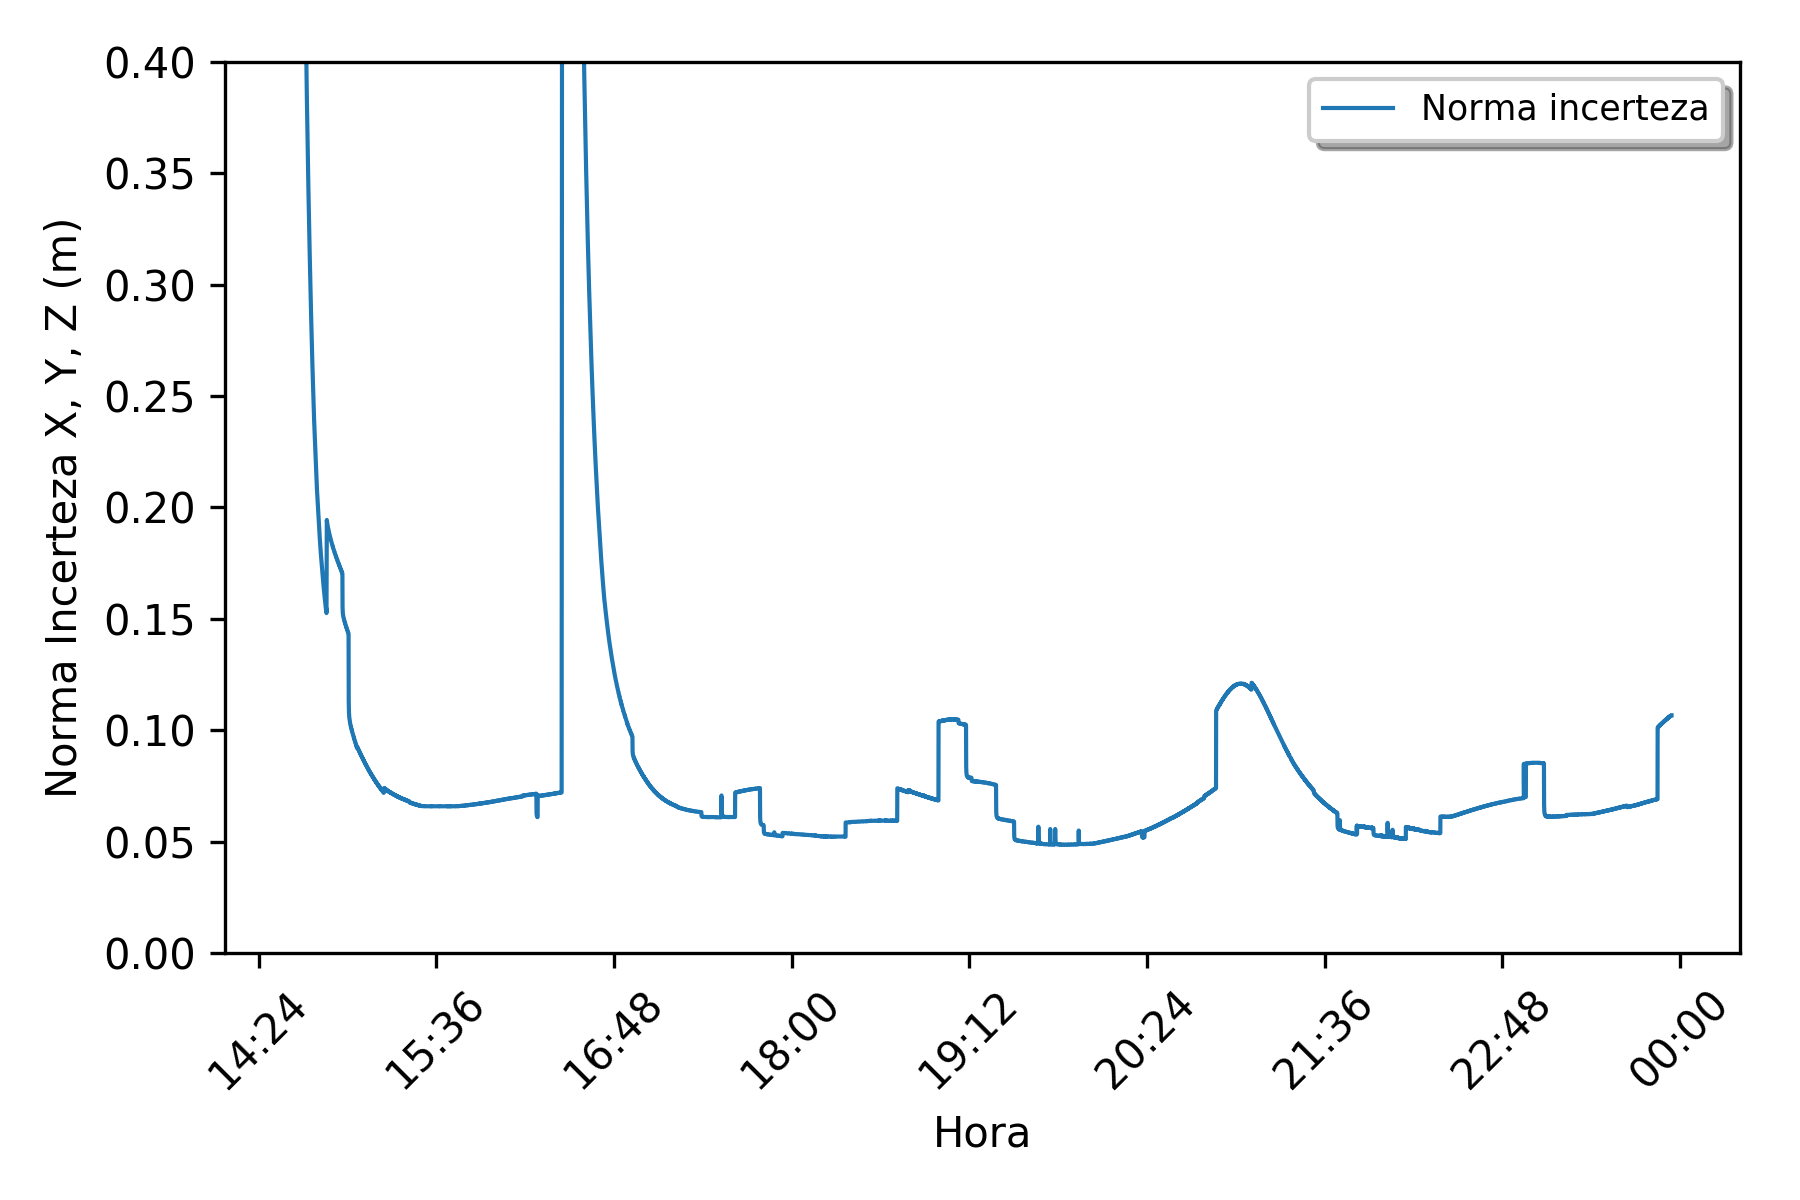
\includegraphics[scale=0.9]{data/Graphics/POAL20650/POAL20650_graphic_uncertainty.png}
\caption{Série temporal RTPPP - Incerteza das coordenadas X, Y, Z.}
\label{incert2}
\end{figure}

O erro médio quadrático deste levantamento foi de $0,205781$. Na fig. \ref{incert2} observa-se que a resultante das incertezas das coordenadas X, Y e Z variou, na maior parte do tempo, entre aproximadamente 5 e 15 cm. 

\begin{figure}[H]
\centering
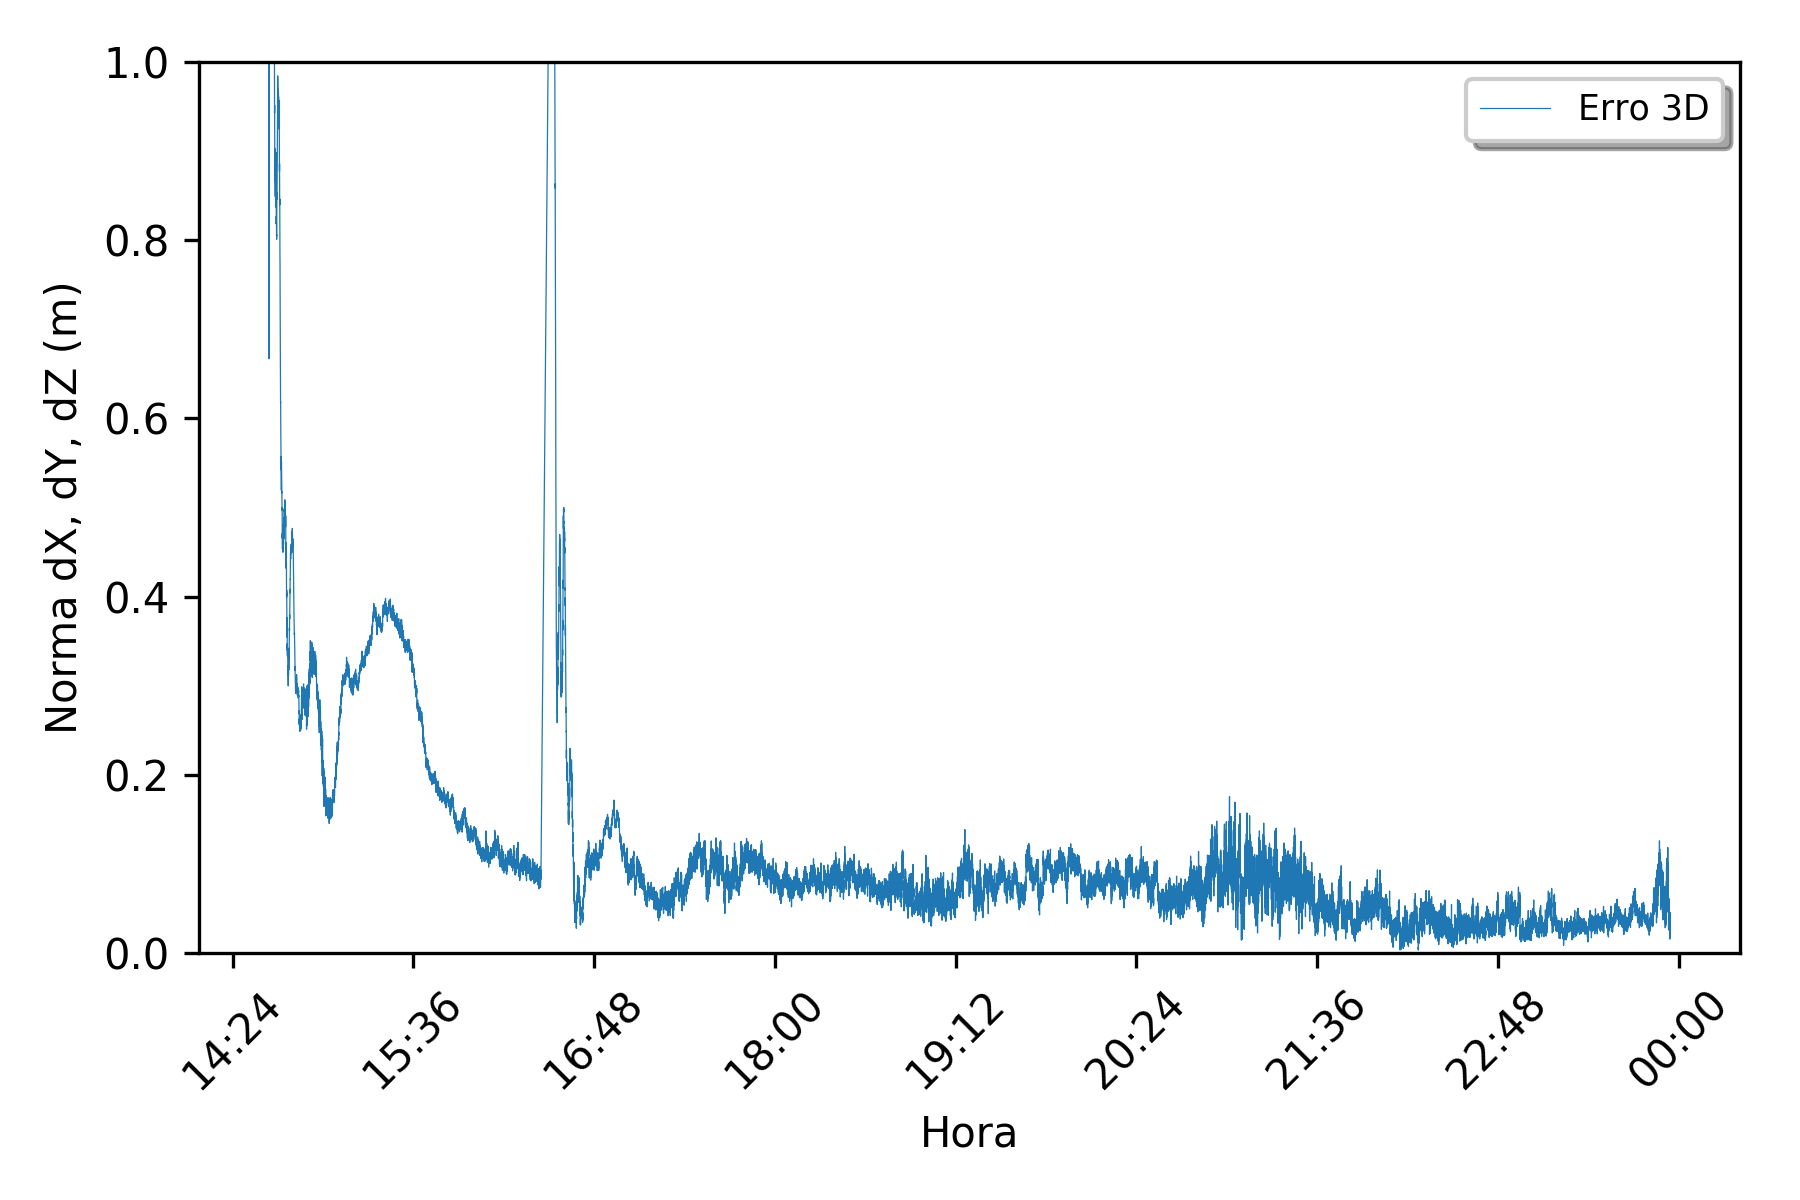
\includegraphics[scale=0.9]{data/Graphics/POAL20650/POAL20650_graphic_result.png}
\caption{Série temporal RTPPP - Norma de dX, dY, dZ.}
\label{}
\end{figure}

\section{RTPPP com GR-5}
\subsection{RTPPP em estação estática}
\label{rtppp_estacao_estatica}
Com o objetivo de atender a proposta de realizar-se um RTPPP utilizando ferramentas de software livre, realizou-se em 17 de setembro de 2019 uma coleta de dados com o receptor GR-5 conectado a um notebook com o software BNC. O receptor estava no marco ''91752'' do IBGE, localizado no terraço do prédio dos fundos do IME. A conexão do receptor com o computador foi feita utilizando um cabo Serial/Porta-COM com um adaptador Porta-COM/USB. A coleta durou aproximadamente 4 horas. A seguir os resultados:

\begin{figure}[H]
\centering
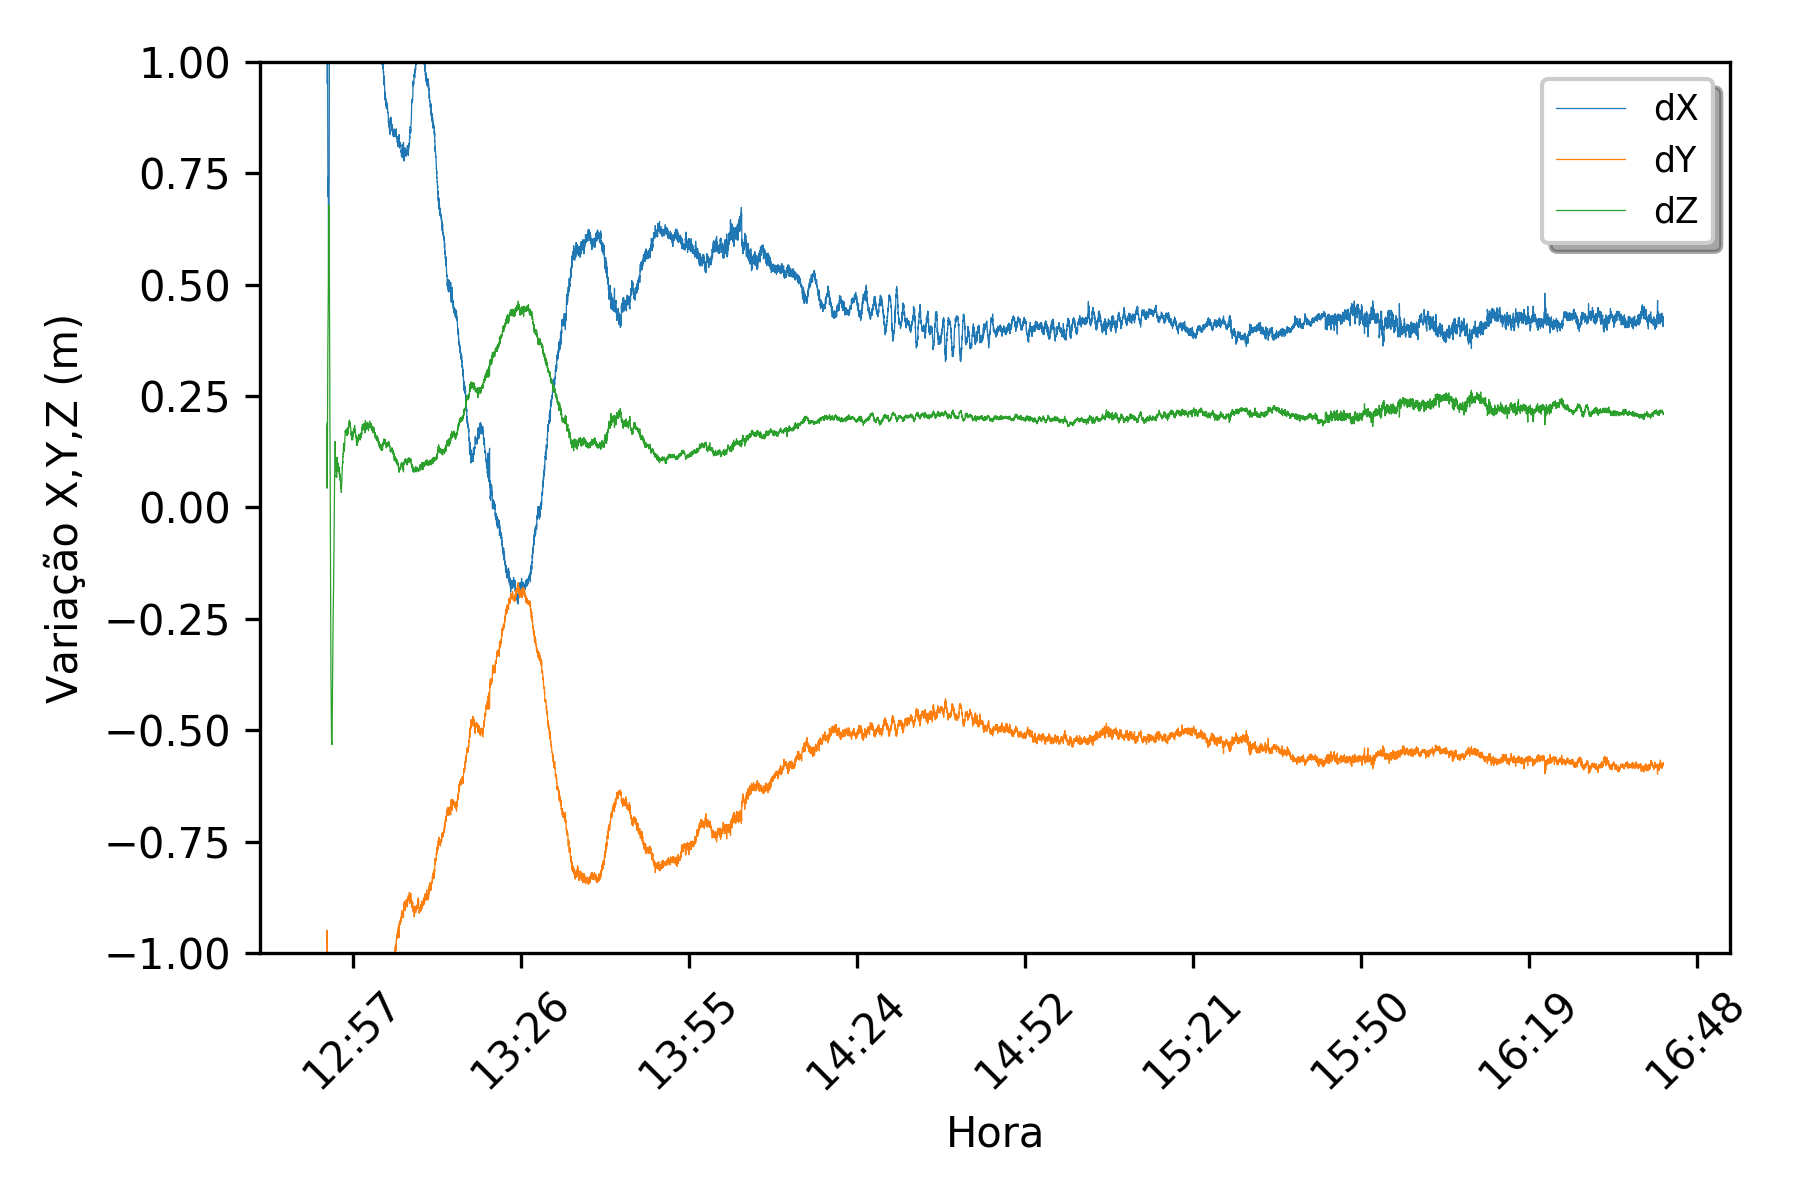
\includegraphics[scale=0.9]{data/Graphics/RJ_T20712/RJ_T20712_graphic_xyz.png}
\caption{Série temporal RTPPP - Resultante dX, dY, dZ.}
\label{}
\end{figure}

As coordenadas utilizadas como referências para o cálculo de dX, dY e dZ foram obtidas a partir da atualização das coordenadas obtidas no descritivo da estação do IBGE. O levantamento foi realizado entre 12h e 16h, sendo que esse é o período de maior atividade solar durante o dia, portanto os efeitos de ionosfera podem ter afetado a convergência do posicionamento.% As coordenadas atualizadas são: X = 4285796.90510288, Y = -4019920.95100773, Z = -2472249.93687366.

\begin{figure}[H]
\centering
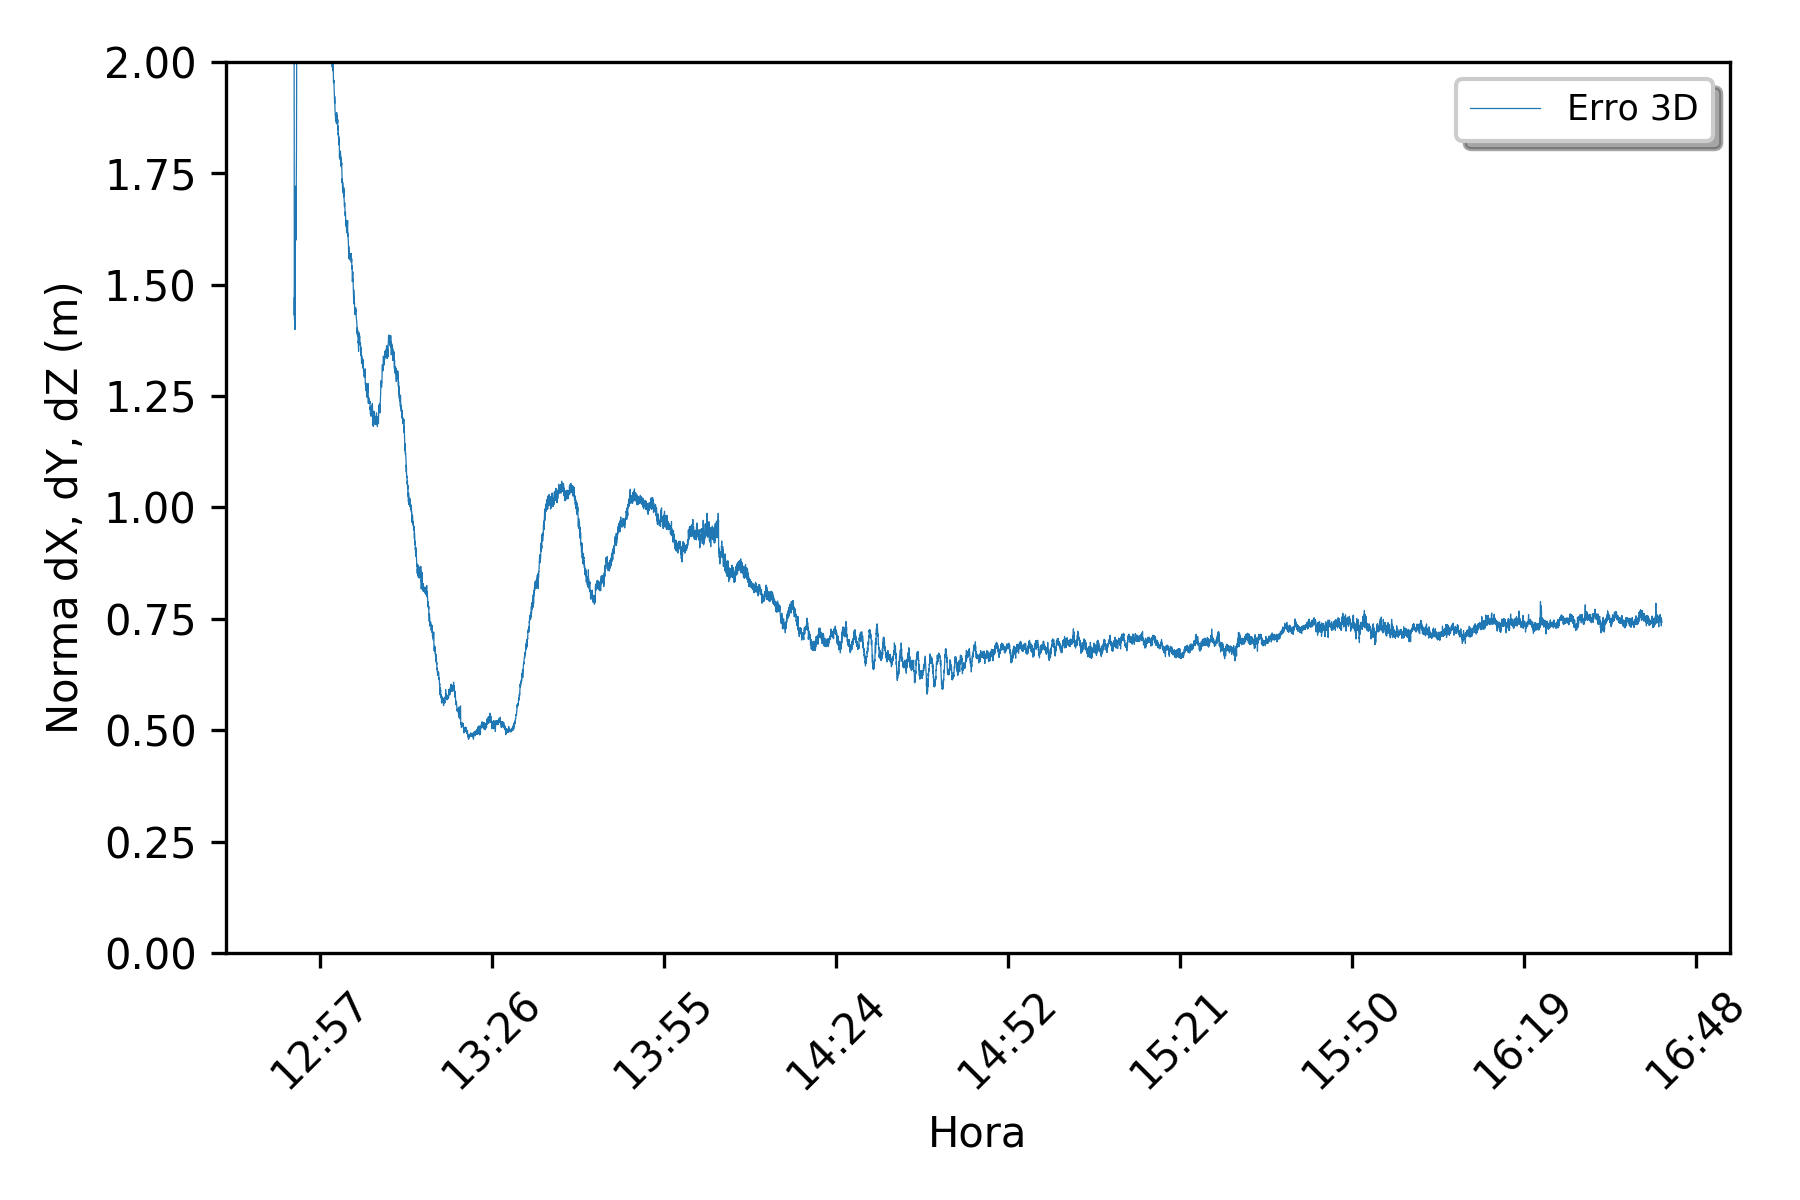
\includegraphics[scale=0.9]{data/Graphics/RJ_T20712/RJ_T20712_graphic_result.png}
\caption{Série temporal RTPPP - Norma de dX, dY, dZ.}
\label{result_20712}
\end{figure}

Na figura \ref{result_20712} é possível observar a resultante de dX, dY e dZ. Utilizando os valores utilizados para construir o gráfico da figura \ref{result_20712} calculou-se o erro médio quadrático que foi de 0,921187 m.

\begin{figure}[H]
\centering
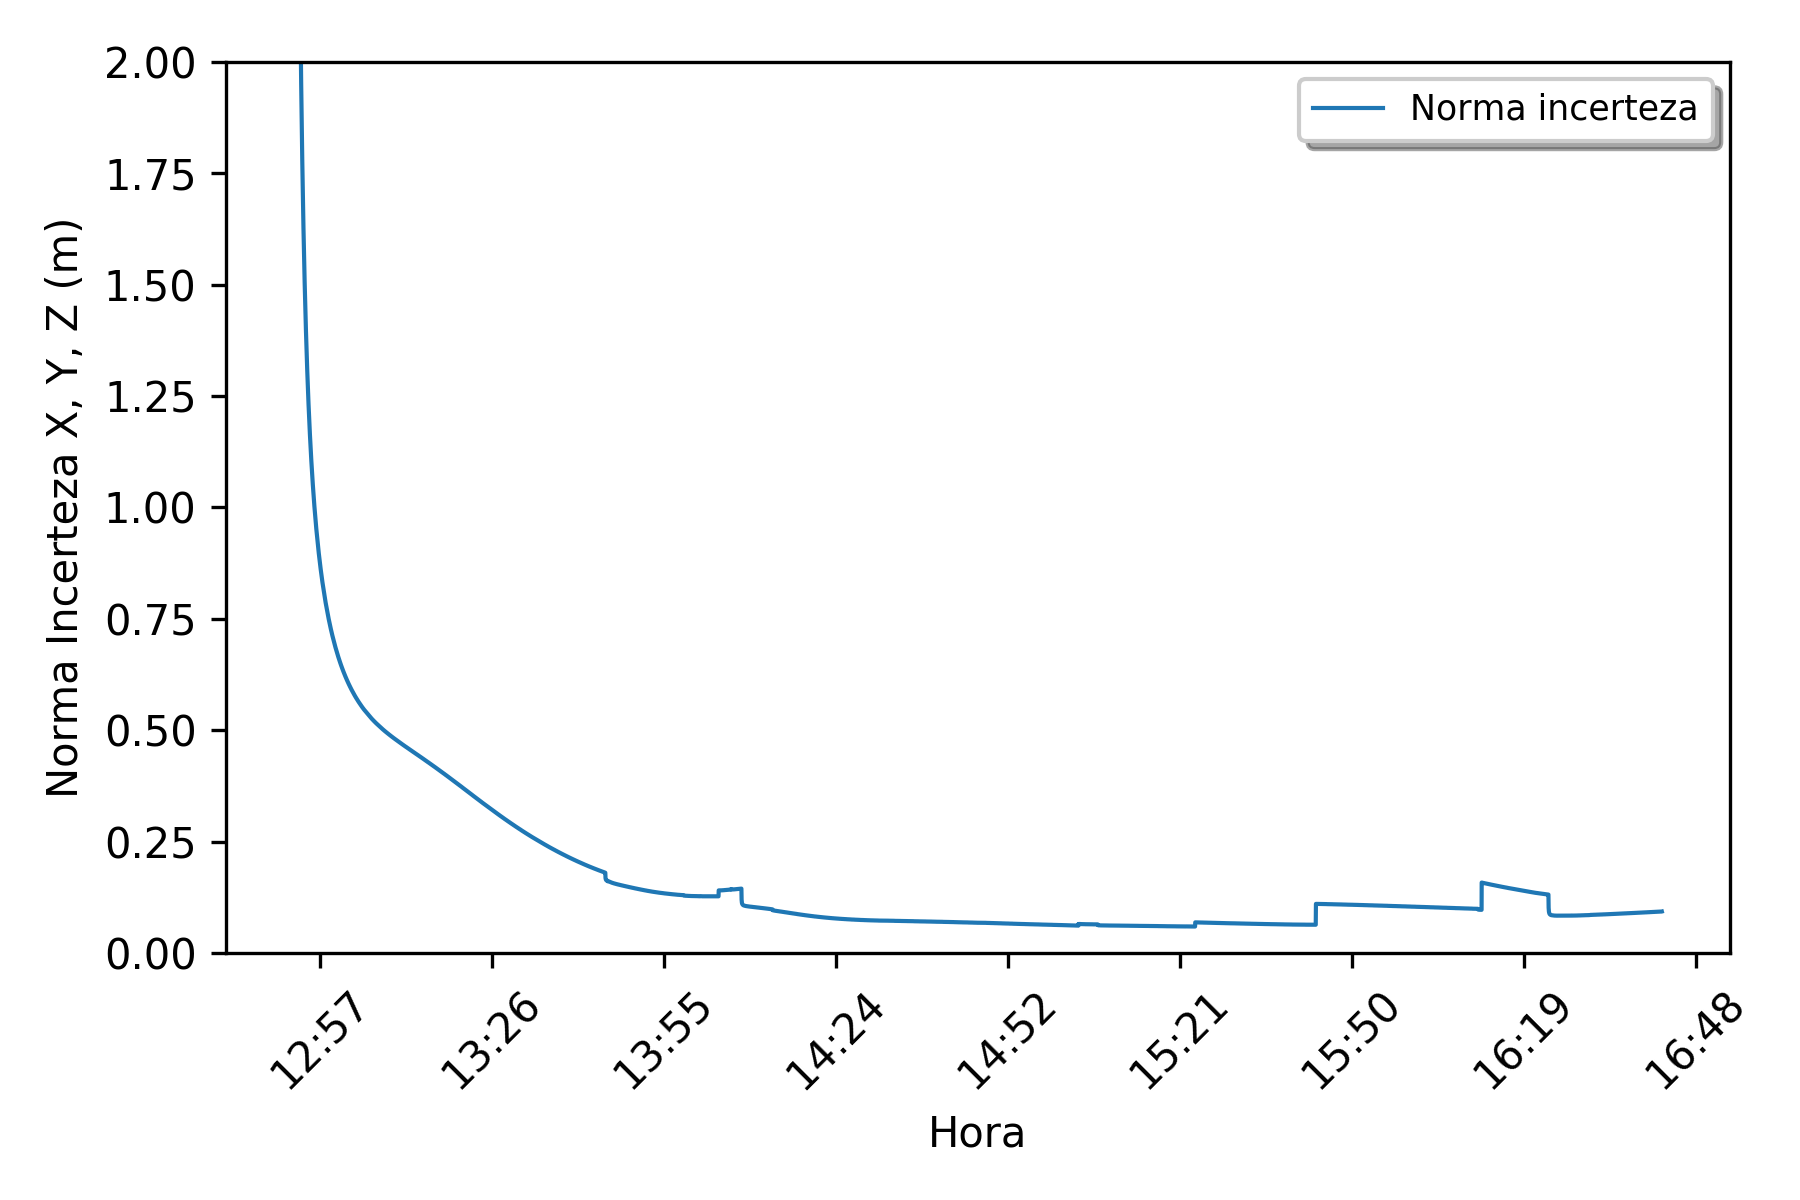
\includegraphics[scale=0.9]{data/Graphics/RJ_T20712/RJ_T20712_graphic_uncertainty.png}
\caption{Série temporal RTPPP - Incerteza das coordenadas X, Y, Z.}
\label{incerteza_20712}
\end{figure}

Na figura \ref{incerteza_20712} é possível observar que a resultante das incertezas converge para valores inferiores a 50 cm em torno de 10 a 15 minutos. Após uma hora a resultante varia de 10 a 20 cm.

Com o intuito de verificar a qualidade do levantamento realizado utilizou-se a ferramenta do IBGE de pós-processamento de dados GNSS \citep{ibge-ppp}, tal ferramenta se utiliza das efemérides ultra-rápidas, rápidas e finais para melhorar a acurácia do posicionamento. No processamento em questão os dados foram inseridos após 36 horas e menos de 11 dias do fim do rastreio, portanto o processamento utilizou-se de efemérides rápidas \citep{ibge_manual_ppp}. Os arquivos RINEX obtidos na medição foram utilizados para o processamento. Com o resultado do processamento comparou-se as coordenadas cartesianas época a época com as coordenadas obtidas em tempo real. A seguir os resultados:

\begin{figure}[H]
\centering
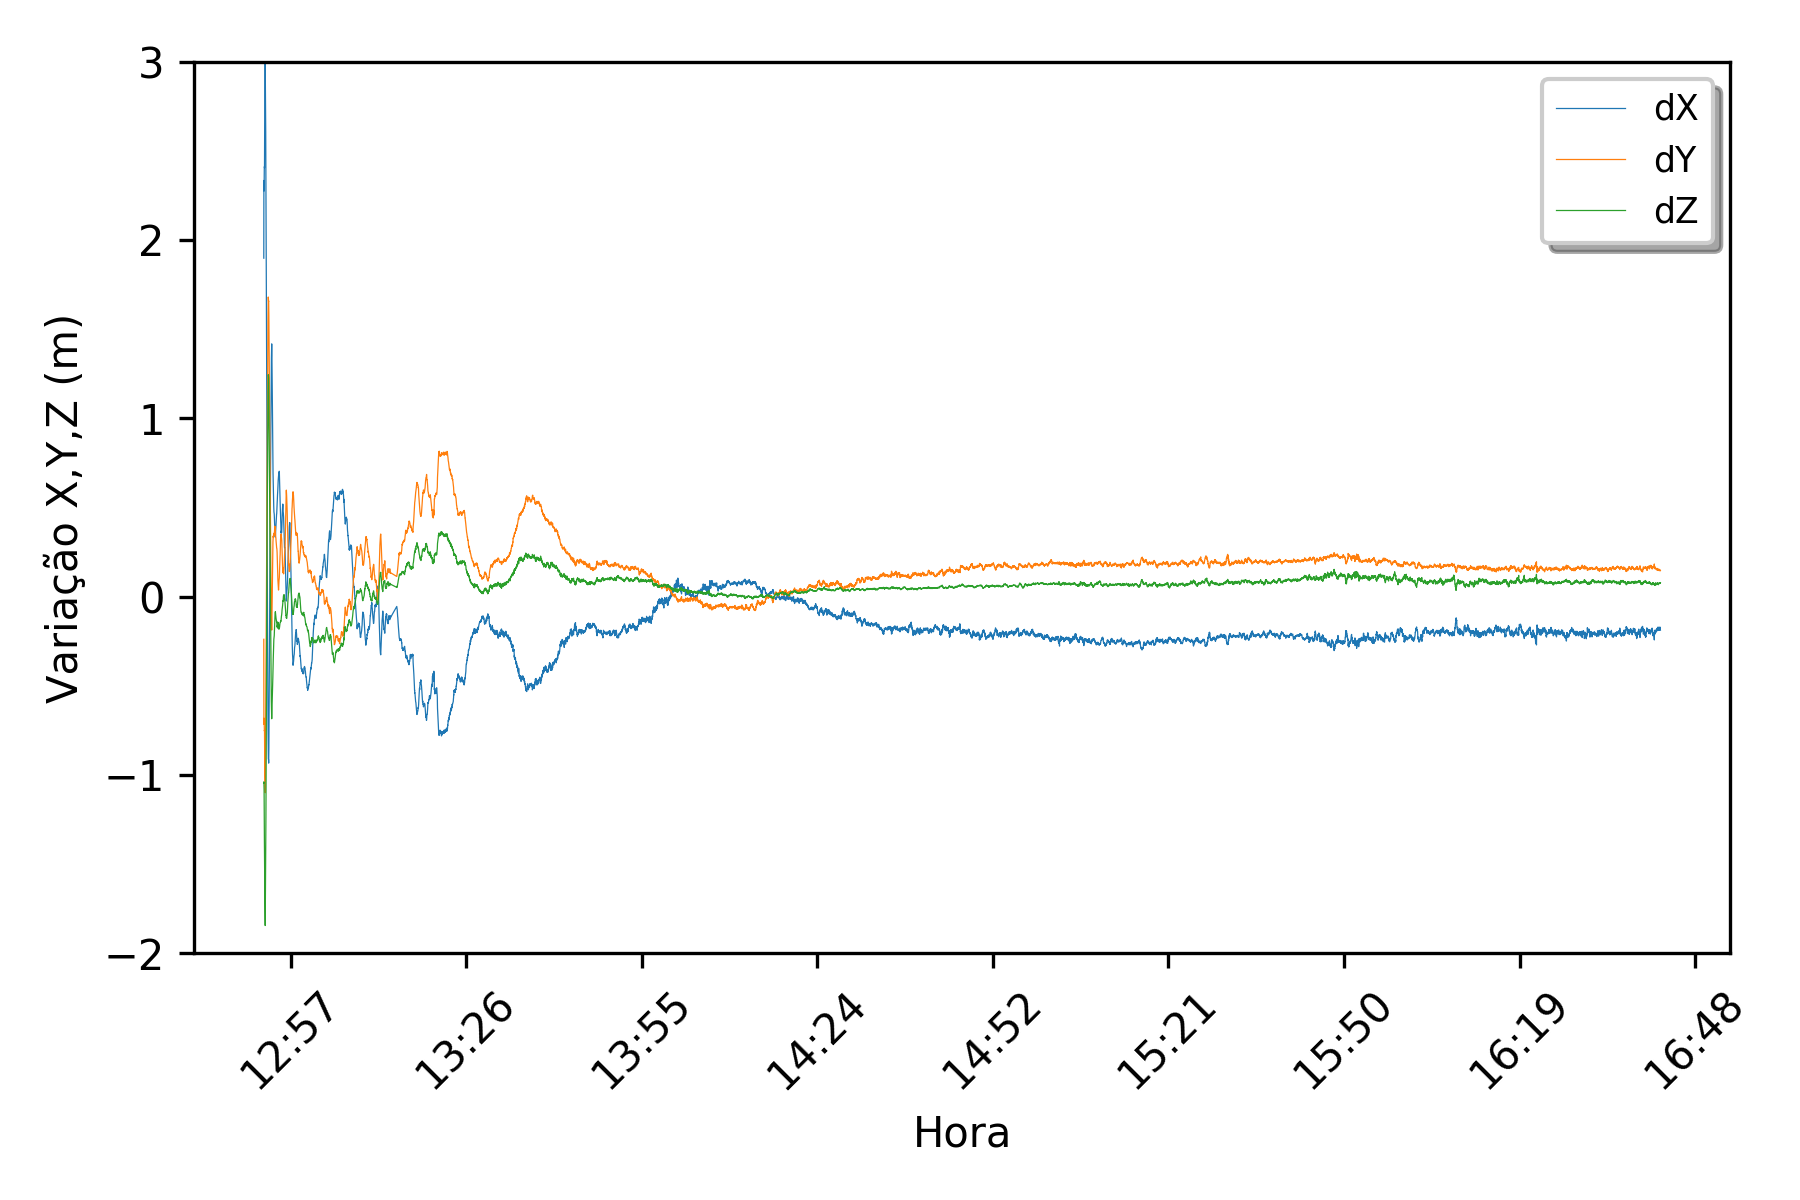
\includegraphics[scale=0.9]{data/Graphics/RJ_T20712/RJ_T20712_comparison_graphic_xyz.png}
\caption{Resultante dX, dY, dZ - Tempo real em comparação com pós-processado do IBGE.}
\label{comp_xyz_20712}
\end{figure}


\begin{figure}[H]
\centering
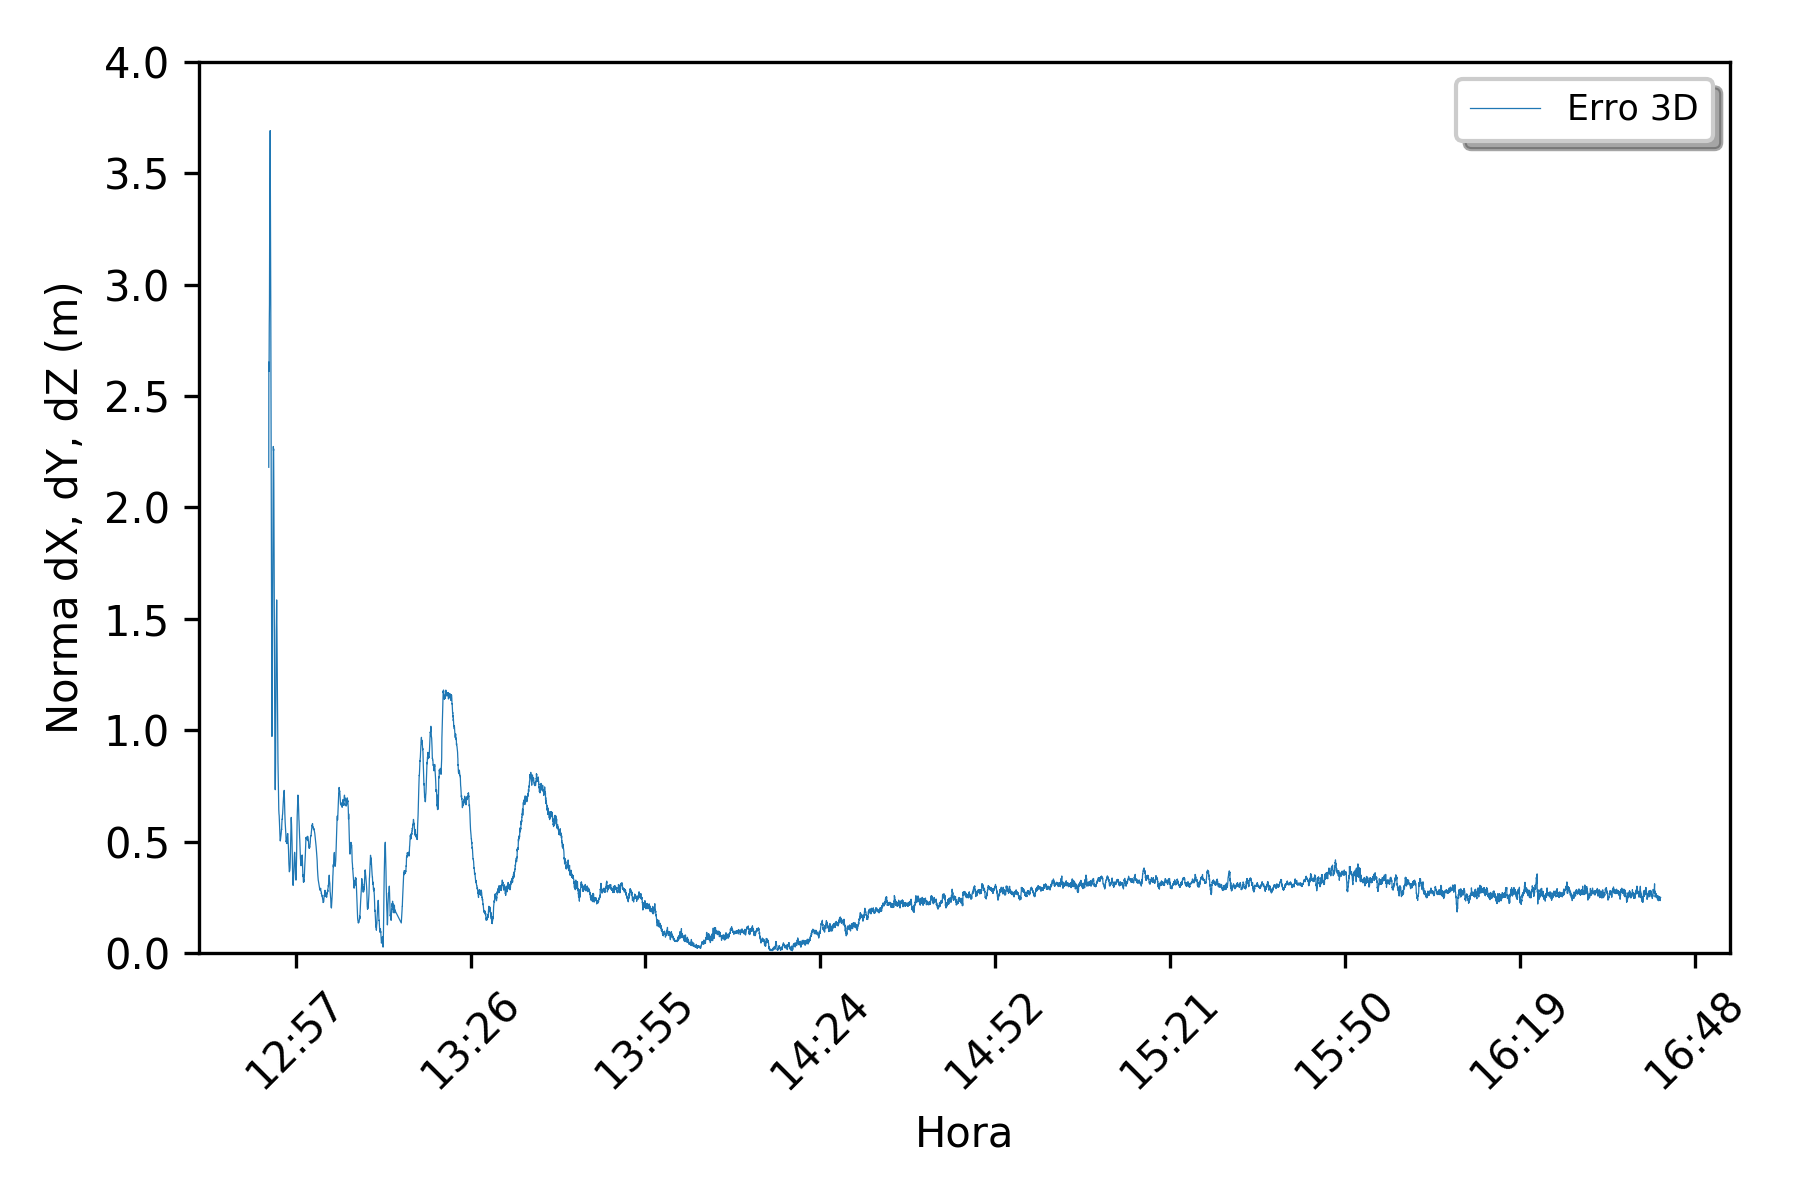
\includegraphics[scale=0.9]{data/Graphics/RJ_T20712/RJ_T20712_comparison_graphic_result.png}
\caption{Norma de dX, dY, dZ - Tempo real em comparação com pós-processado do IBGE.}
\label{comp_norma_20712}
\end{figure}

Pode-se observar na figura \ref{comp_xyz_20712} que os valores de dX, dY e dZ apresentam uma queda brusca de valores após os primeiros minutos de levantamento. Na figura \ref{comp_norma_20712} observa-se que na maior parte do levantamento, após uma hora de coleta, os valores da norma de dX, dY e dZ não são superiores a 50 cm e tem-se ainda que o erro quadrático médio é de 0,385575 m.

\subsection{RTPPP em estação cinemática}

Com o intuito de consolidar o posicionamento preciso em tempo real utilizando plataformas livres, realizou-se um levantamento na Praça Gen. Tibúrcio, Rio de Janeiro - RJ com um \textit{notebook} com software BNC conectado ao receptor GR-5 via porta serial. O \textit{notebook} estava conectado à internet via 4G e portanto recebendo as correções necessárias para a realização do PPP. As observáveis GNSS foram recebidas pela conexão com o receptor via porta serial. É possível observar nas figuras \ref{incerteza_20721}, \label{comp_xyz_20721} e \label{comp_norma_20721} que o tempo de levantamento foi pouco levando em consideração o tempo ideal para a convergência. A situação ideal é permanecer durante alguns minutos em um ponto estático e em seguida iniciar o levantamento; tal conduta não pôde ser seguida devido a limitações técnicas do \textit{notebook} utilizado. 

O traçado percorrido pelo levantamento pode ser observado pela linha branca da figura \ref{rtppp_praca}.

\begin{figure}[H]
\centering
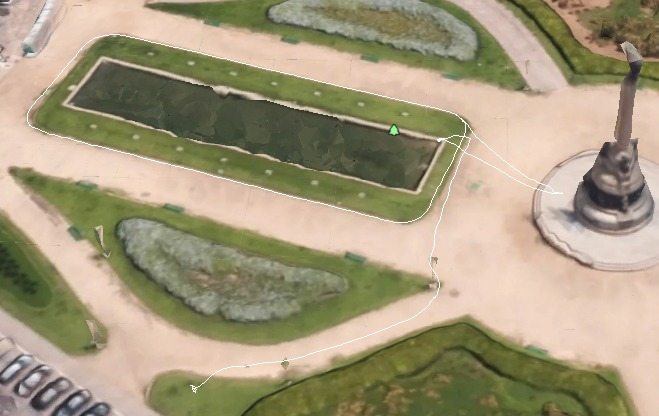
\includegraphics[scale=0.6]{pfc_pdf_files/img/rtppp_praca.jpeg}
\caption{Traçado levantamento RTPPP.}
\label{rtppp_praca}
\end{figure}

Na figura \ref{incerteza_20721} é possível observar que a resultante das incertezas converge para valores inferiores a 50 cm em menos de 10 minutos.

\begin{figure}[H]
\centering
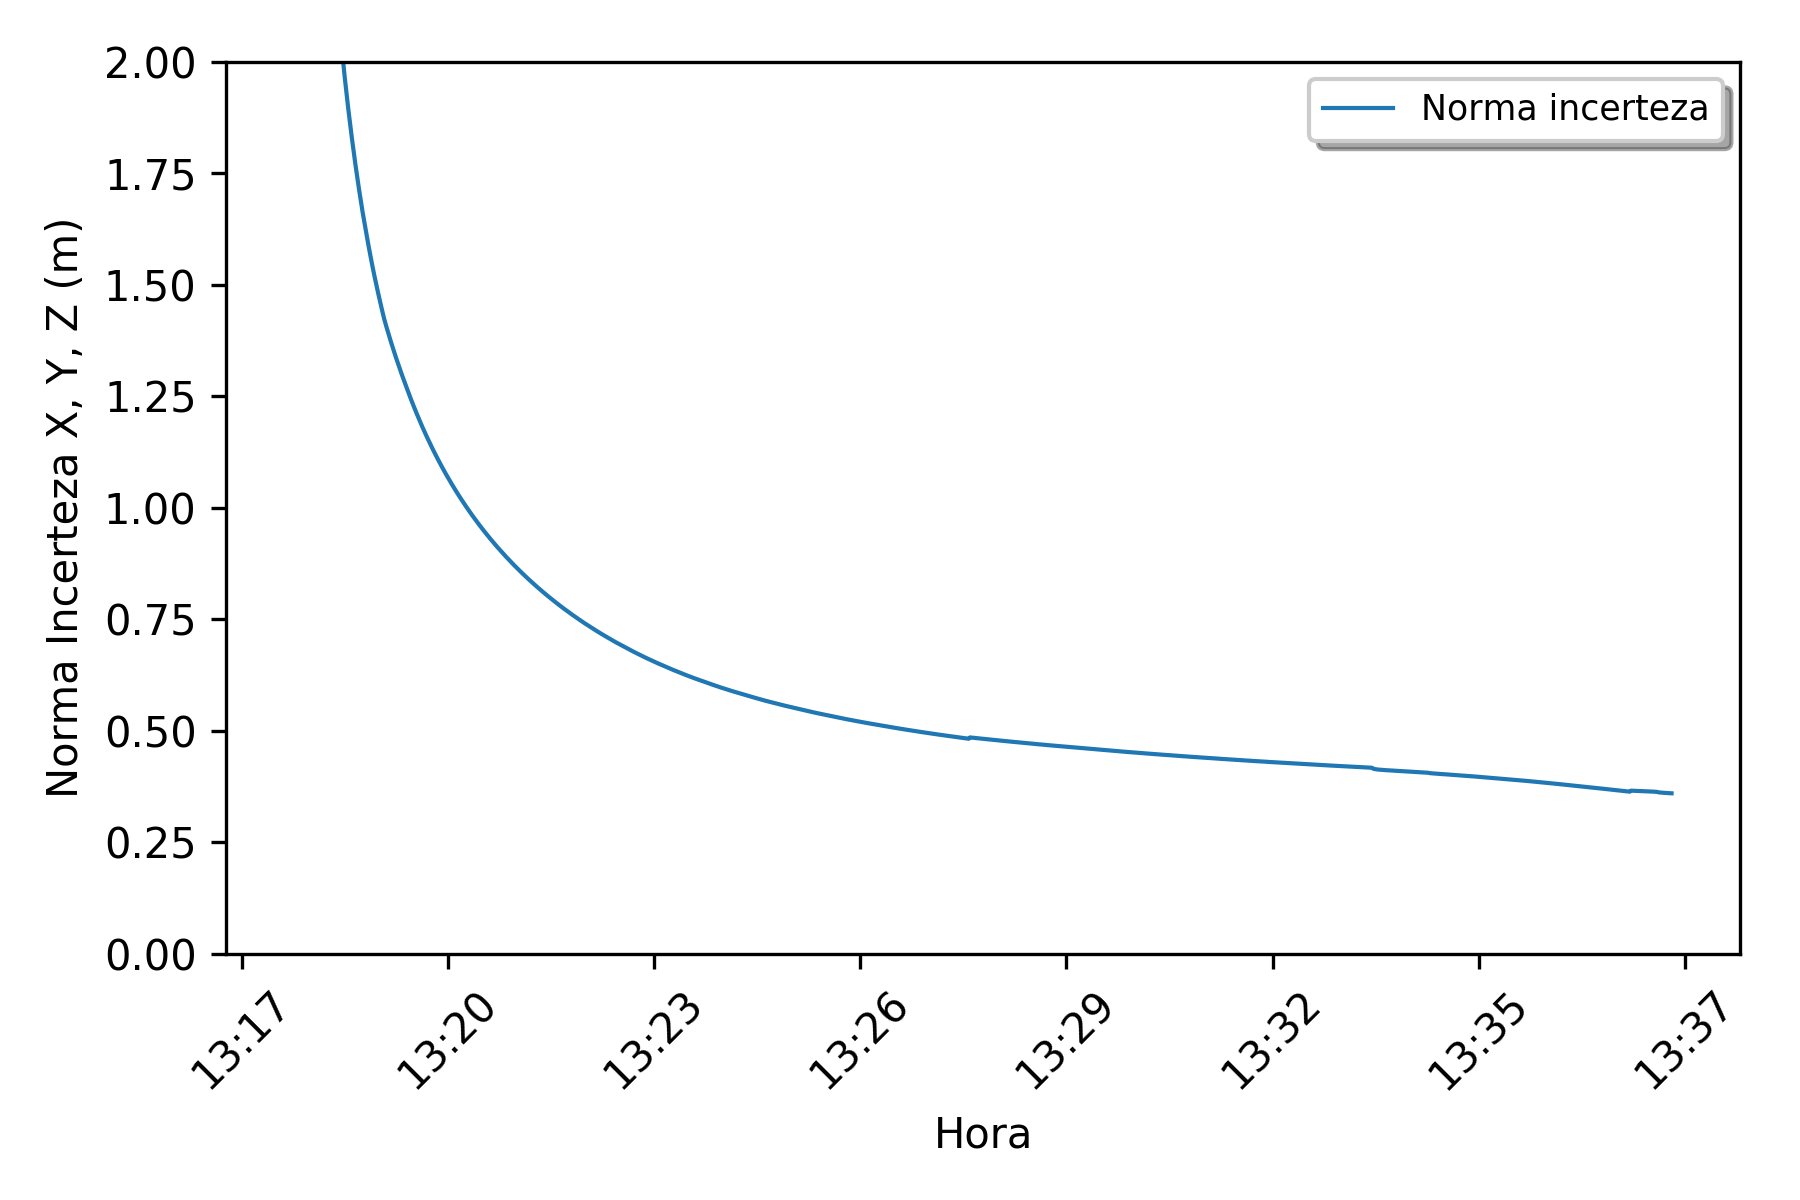
\includegraphics[scale=0.9]{data/Graphics/RJ_T20721/RJ_T20721_graphic_uncertainty.png}
\caption{Série temporal RTPPP - Incerteza das coordenadas X, Y, Z.}
\label{incerteza_20721}
\end{figure}


Assim como na seção \ref{rtppp_estacao_estatica} utilizou-se a ferramenta do IBGE de pós-processamento para avaliar a qualidade do levantamento. O erro quadrático médio encontrado foi de 2,446697 m. A seguir os resultados:

\begin{figure}[H]
\centering
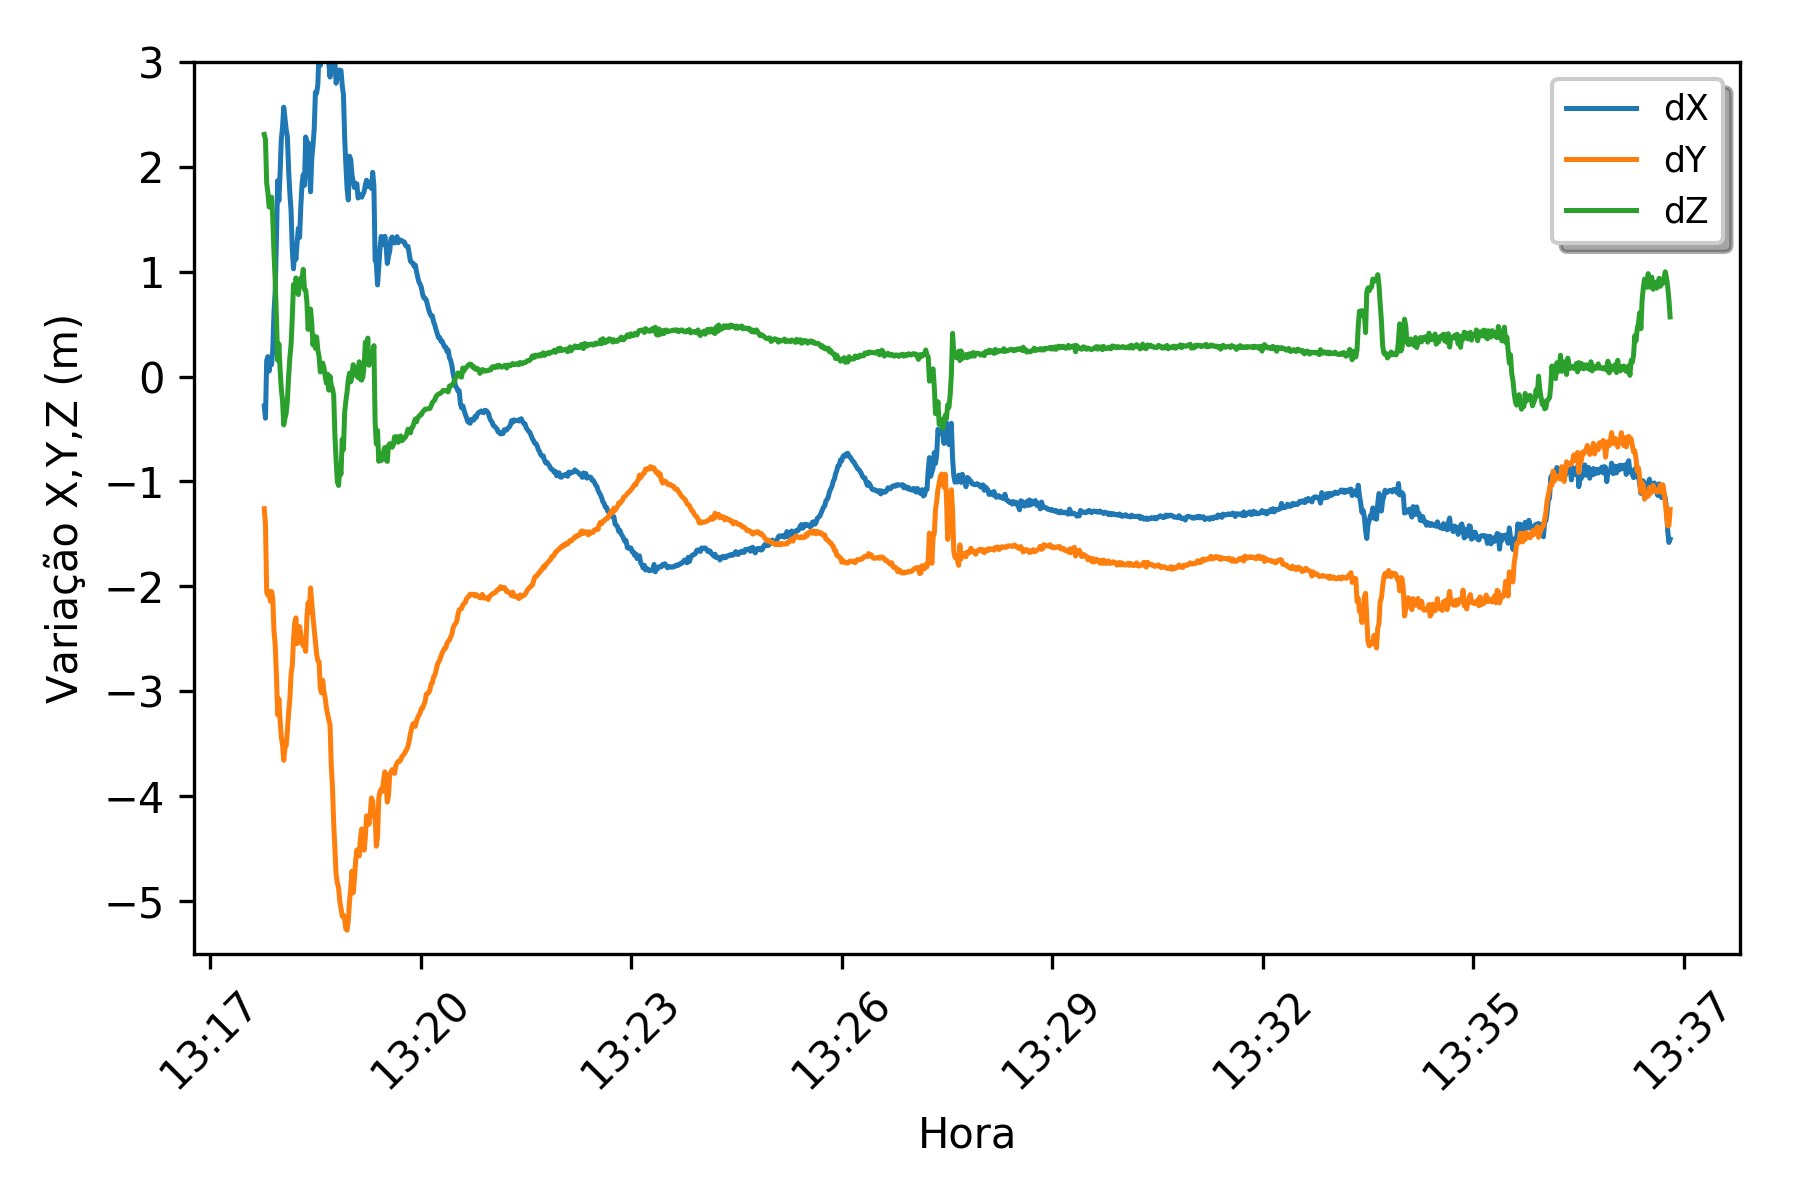
\includegraphics[scale=0.9]{data/Graphics/RJ_T20721/RJ_T20721_comparison_graphic_xyz.png}
\caption{Resultante dX, dY, dZ - Tempo real em comparação com pós-processado do IBGE.}
\label{comp_xyz_20721}
\end{figure}


\begin{figure}[H]
\centering
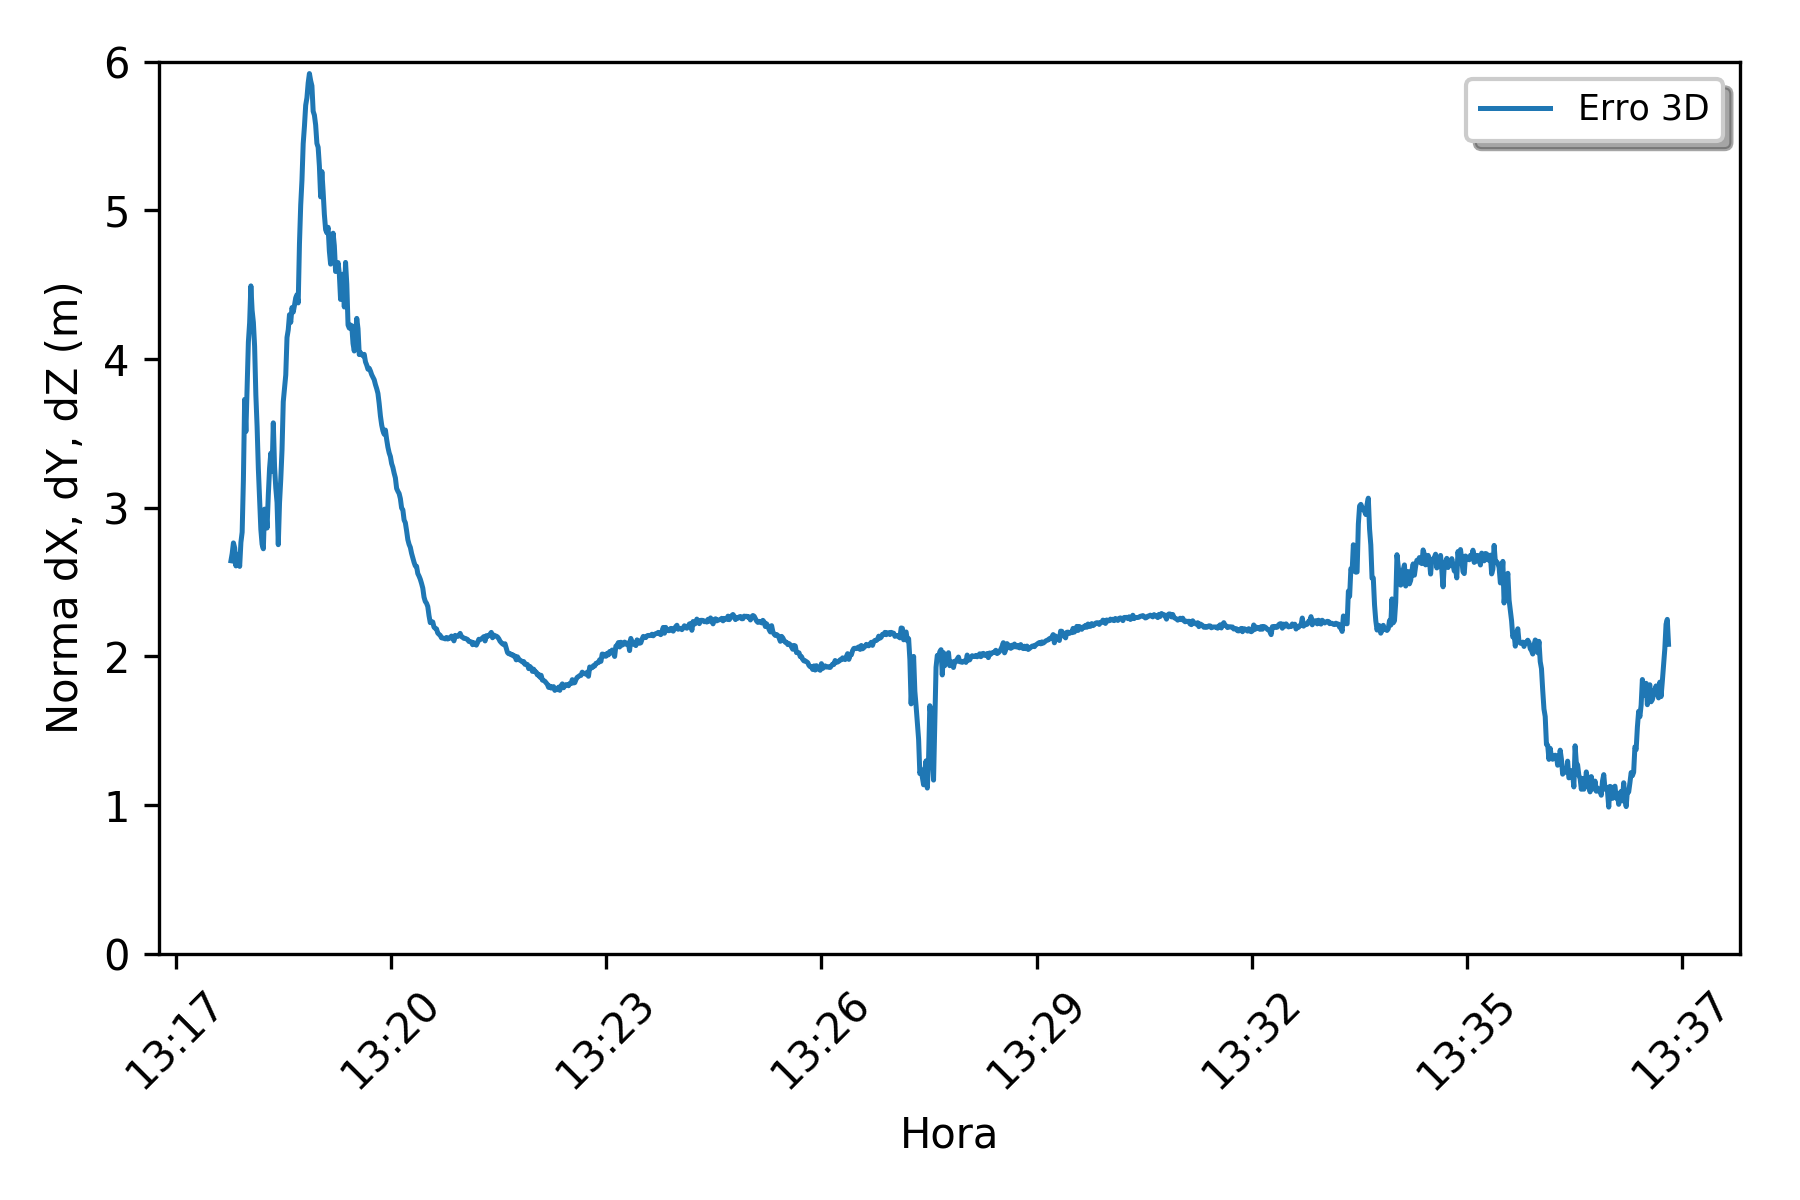
\includegraphics[scale=0.9]{data/Graphics/RJ_T20721/RJ_T20721_comparison_graphic_result.png}
\caption{Norma de dX, dY, dZ - Tempo real em comparação com pós-processado do IBGE.}
\label{comp_norma_20721}
\end{figure}



\section{PPP-RTK}
Para a realização do método PPP-RTK utilizou-se o software ''PPP-Wizard''. Para fim de comparação entre o RTPPP, o qual utiliza solução \textit{float} de ambiguidades, e o PPP-RTK, o qual utiliza solução \textit{fixa} de ambiguidades, realizou-se, durante 24 horas, coleta de dados referente a estação POAL. A seguir os resultados:



\begin{figure}[H]
\centering
\subfigure[PPP-RTK\label{}]{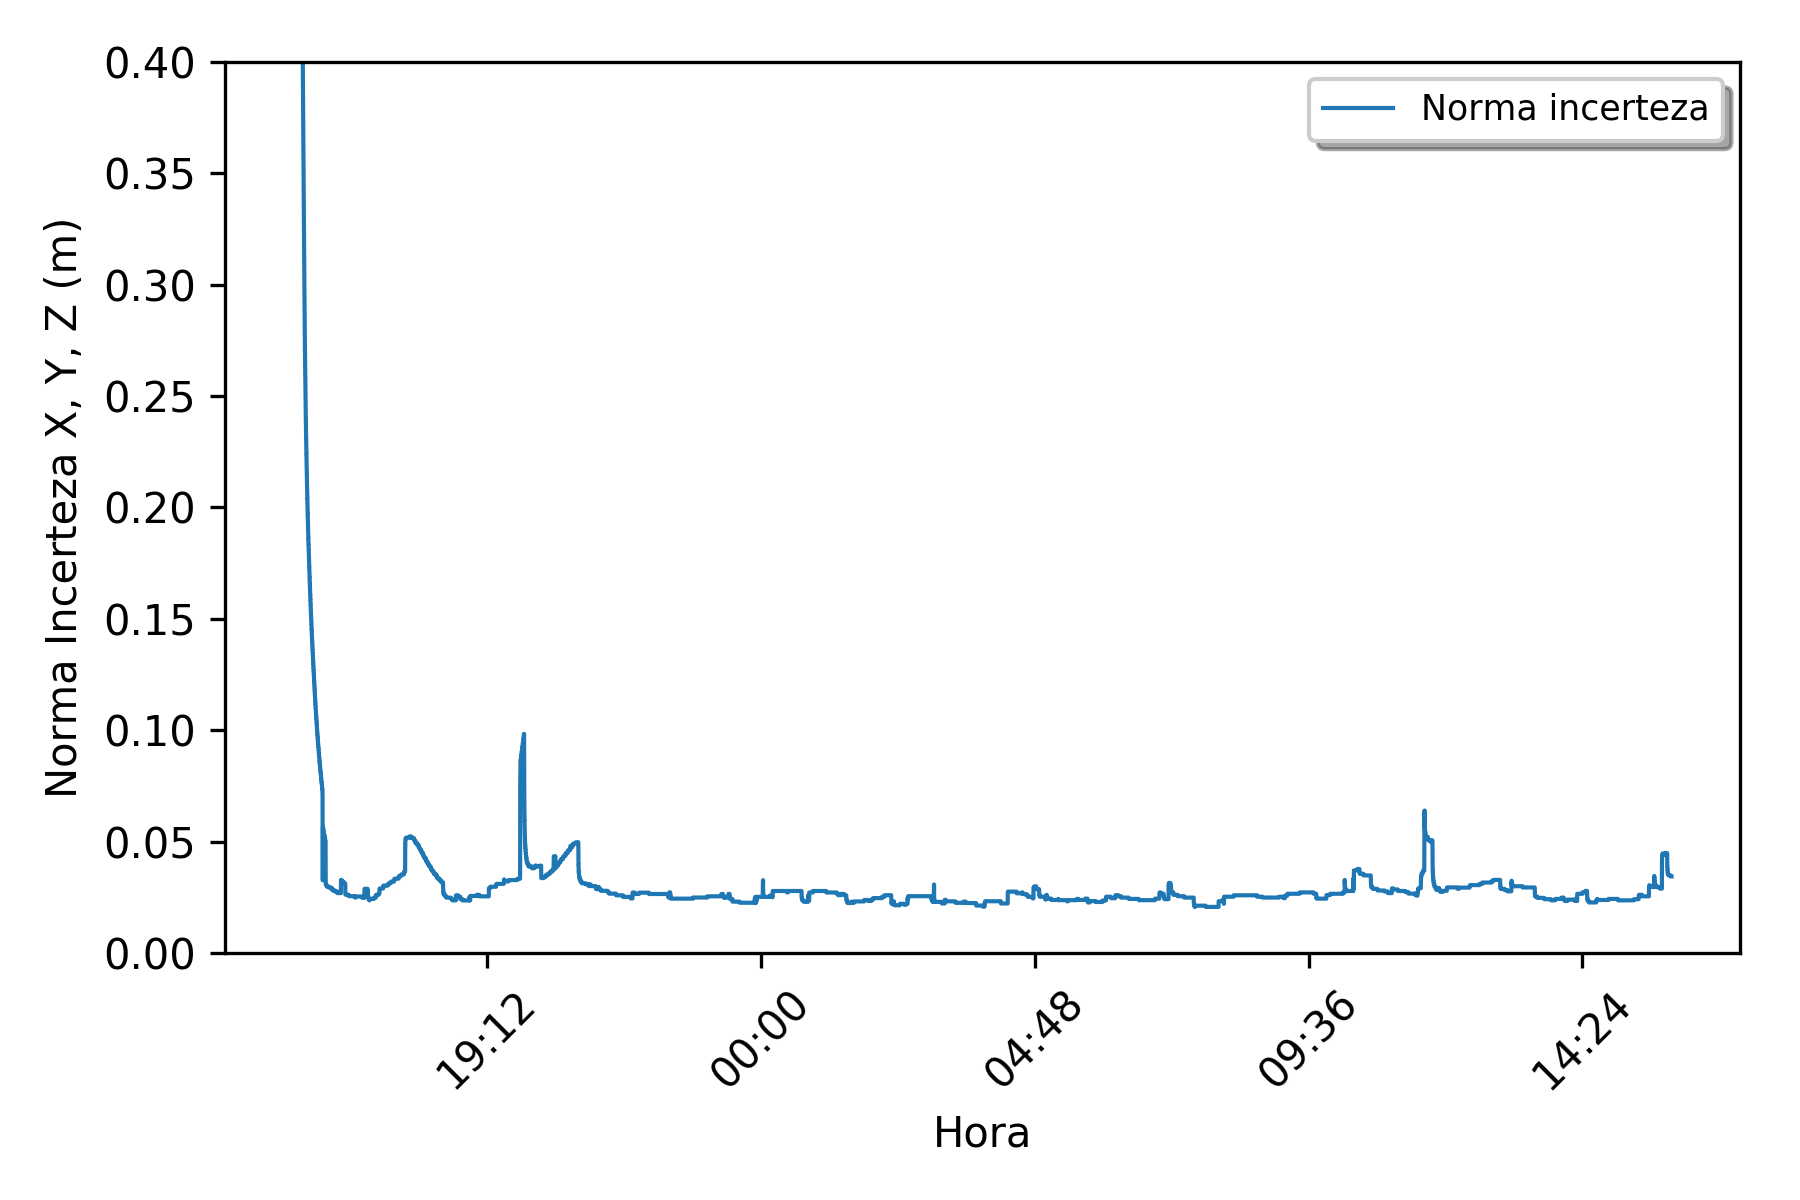
\includegraphics[scale=0.7]{data/Graphics/POAL001_ppp_wizard/POAL001_ppp_wizard_graphic_uncertainty.png}}
\subfigure[RTPPP\label{}]{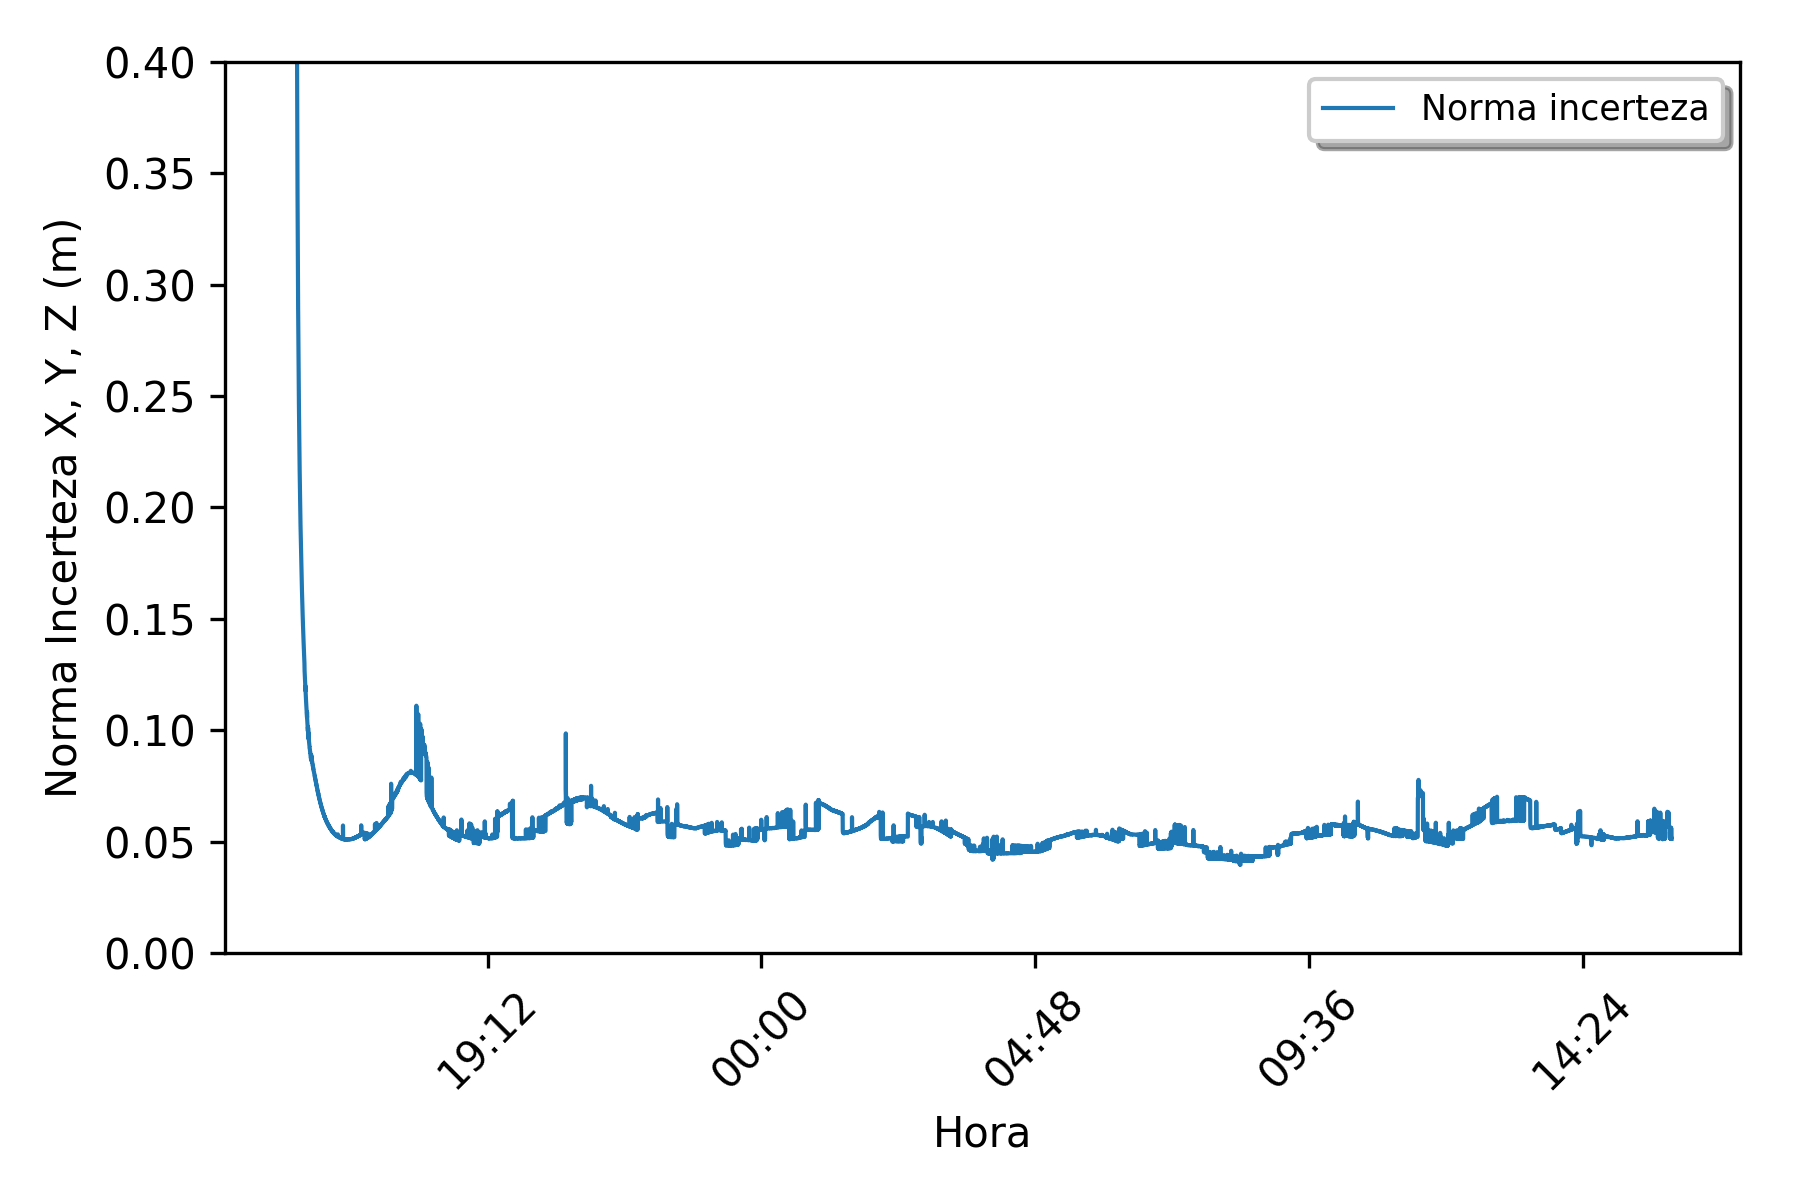
\includegraphics[scale=0.7]{data/Graphics/POAL20716/POAL20716_graphic_uncertainty.png}}
\caption{Comparação das incertezas entre RTPPP e PPP-RTK}
\label{comparacao_incert}
\end{figure}

Pode-se observar na figura \ref{comparacao_incert} que, como esperado, a resultante incerteza varia em valores menores quando se utilizada a solução fixa de ambiguidades. Ao utilizar-se o método PPP-RTK os valores variam menos e em torno de 3 cm, enquanto que no RTPPP os valores variam acima de 5 cm e apresentam maior variação.

\begin{figure}[H]
\centering
\subfigure[PPP-RTK\label{}]{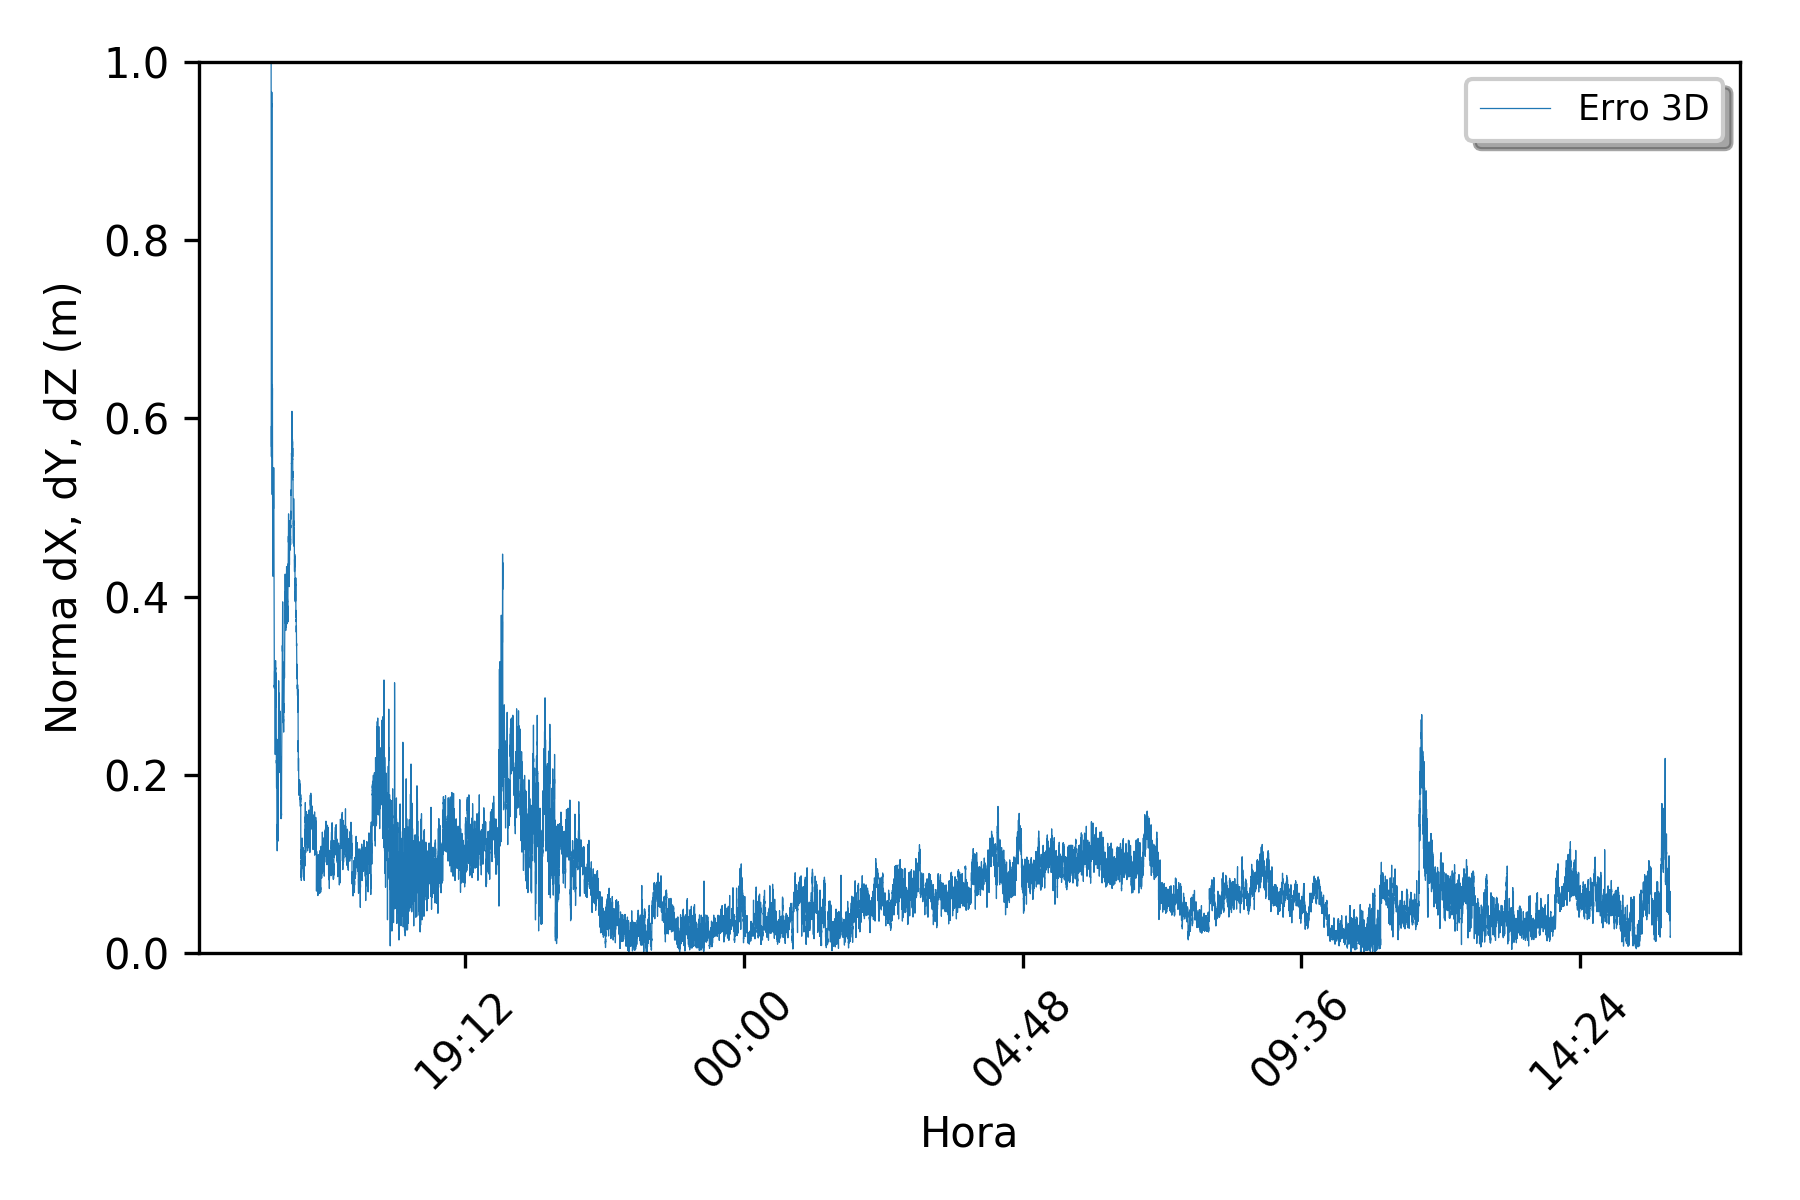
\includegraphics[scale=0.7]{data/Graphics/POAL001_ppp_wizard/POAL001_ppp_wizard_graphic_result.png}}
\subfigure[RTPPP\label{}]{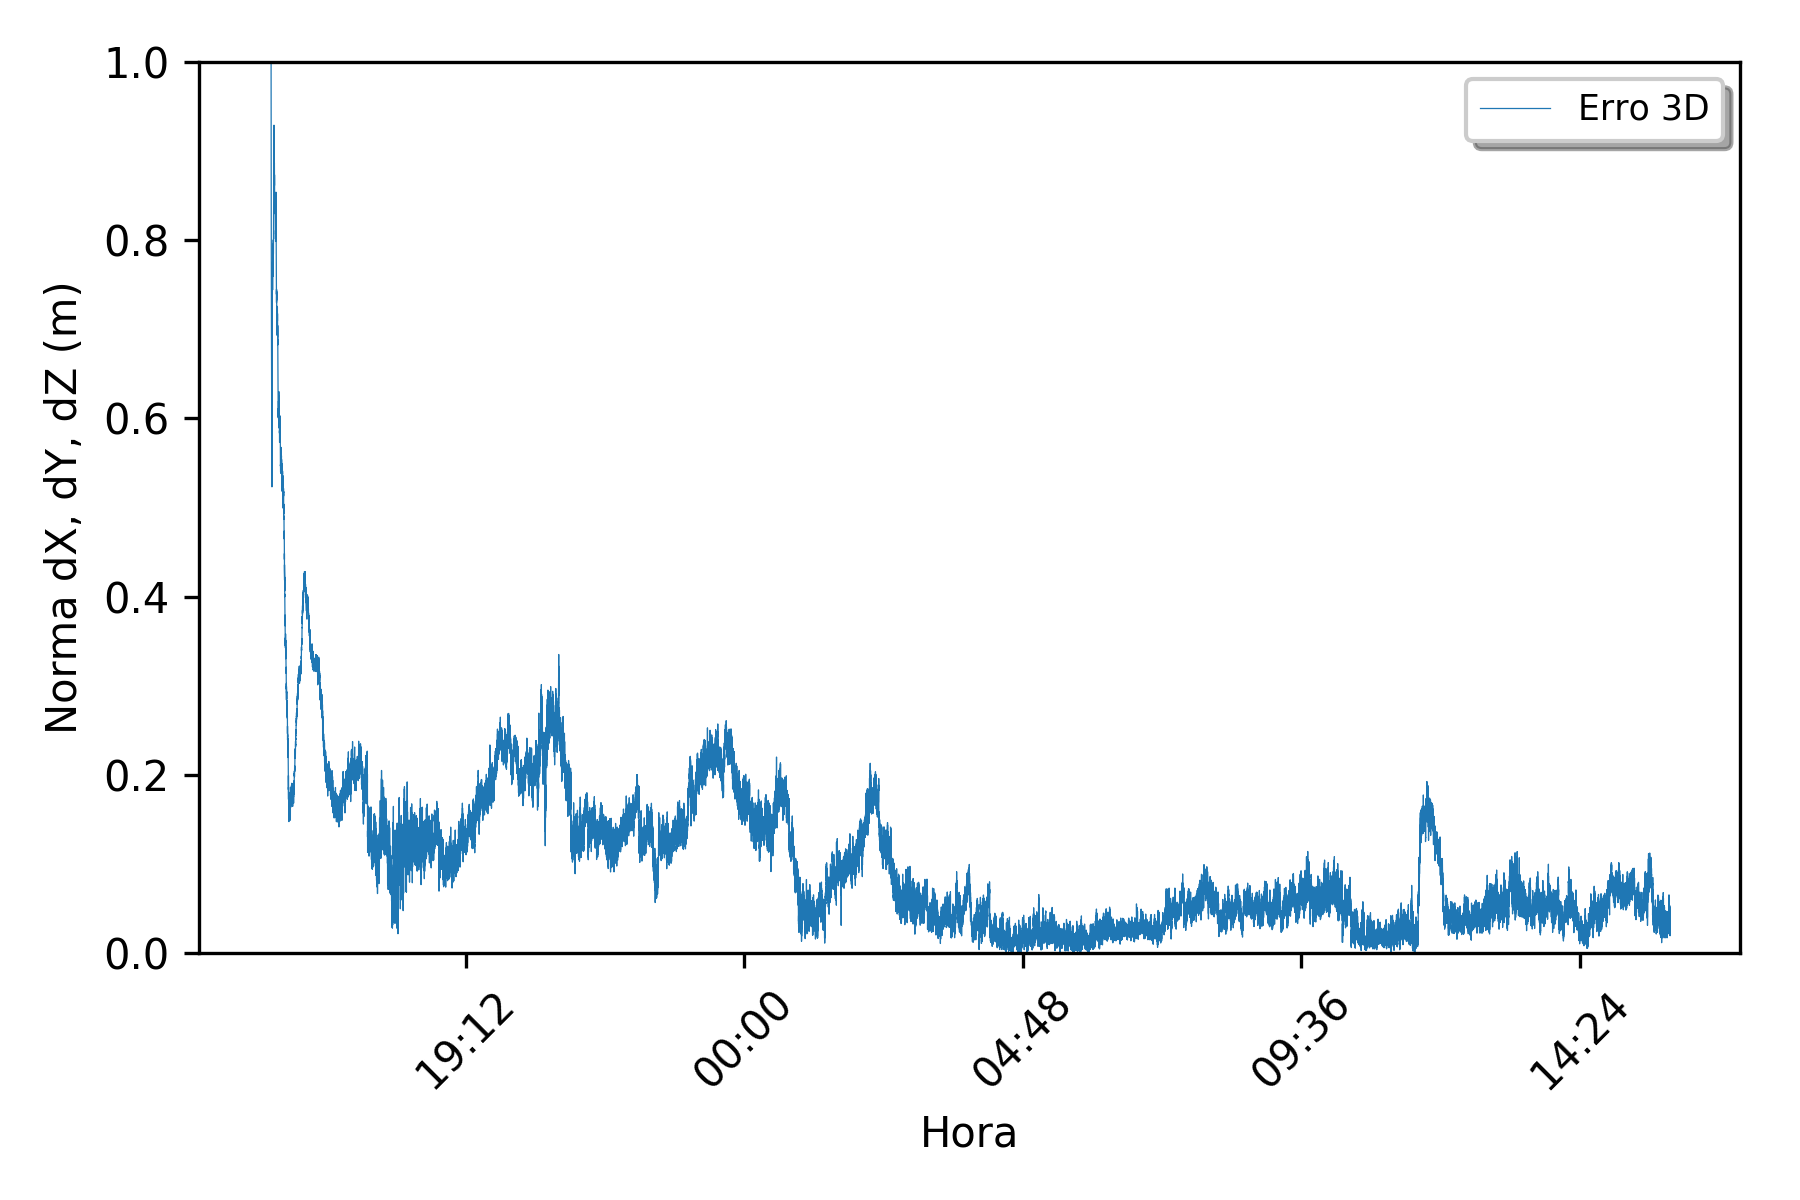
\includegraphics[scale=0.7]{data/Graphics/POAL20716/POAL20716_graphic_result.png}}
\caption{Comparação normas de dX, dY e dZ entre RTPPP e PPP-RTK}
\label{comparacao_xyz}
\end{figure}

Os erros quadráticos médios encontrados foram: para o PPP-RTK - 0,1571640 m; para o RTPPP 0,155435 m. Na figura \ref{comparacao_xyz} é possível observar que ao utilizar o RTPPP a resultante de dX, dY e dZ é ligeiramente maior que ao utilizar o PPP-RTK. Ainda ao analisar a mesma figura é possível verificar que no PPP-RTK os valores alcançam a marca de 10cm em tempo consideravelmente mais rápido do que o RTPPP.

\section{RTK}
Com o objetivo de realizar as primeiras configurações no receptor GR-5, bem como entender corretamente seu funcionamento, realizou-se um RTK no prédio frontal do Instituto Militar de Engenharia, foram obtidos os pontos conforme figura a seguir:

\begin{figure}[H]
\centering
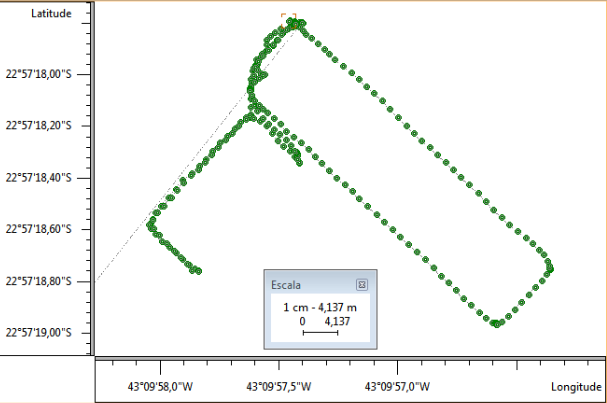
\includegraphics[scale=0.55]{img/rtk/mapa_rtk.png}
\caption{Pontos obtidos com levantamento RTK.}
\label{}
\end{figure}

